\documentclass[10pt,letterpaper]{article}
\usepackage[top=0.85in,left=2.75in,footskip=0.75in]{geometry}

% amsmath and amssymb packages, useful for mathematical formulas and symbols
\usepackage{amsmath,amssymb}

% Use adjustwidth environment to exceed column width (see example table in text)
\usepackage{changepage}

% Use Unicode characters when possible
%\usepackage[utf8x]{inputenc}

% textcomp package and marvosym package for additional characters
\usepackage{textcomp,marvosym}


% Use nameref to cite supporting information files (see Supporting Information section for more info)
\usepackage{nameref,hyperref}

% line numbers
\usepackage[right]{lineno}

% ligatures disabled
\usepackage{microtype}
\DisableLigatures[f]{encoding = *, family = * }

% color can be used to apply background shading to table cells only
\usepackage[table]{xcolor}

% create "+" rule type for thick vertical lines
\newcolumntype{+}{!{\vrule width 2pt}}

% create \thickcline for thick horizontal lines of variable length
\newlength\savedwidth
\newcommand\thickcline[1]{%
  \noalign{\global\savedwidth\arrayrulewidth\global\arrayrulewidth 2pt}%
  \cline{#1}%
  \noalign{\vskip\arrayrulewidth}%
  \noalign{\global\arrayrulewidth\savedwidth}%
}

% \thickhline command for thick horizontal lines that span the table
\newcommand\thickhline{\noalign{\global\savedwidth\arrayrulewidth\global\arrayrulewidth 2pt}%
\hline
\noalign{\global\arrayrulewidth\savedwidth}}


% Remove comment for double spacing
%\usepackage{setspace}
%\doublespacing

% Text layout
\raggedright
\setlength{\parindent}{0.5cm}
\textwidth 5.25in
\textheight 8.75in

% Bold the 'Figure #' in the caption and separate it from the title/caption with a period
% Captions will be left justified
\usepackage[aboveskip=1pt,labelfont=bf,labelsep=period,justification=raggedright,singlelinecheck=off]{caption}
\renewcommand{\figurename}{Fig}

% Use the PLoS provided BiBTeX style
%\bibliographystyle{plos2015}

% Header and Footer with logo
\usepackage{lastpage,fancyhdr,graphicx}
\usepackage{epstopdf}
\pagestyle{myheadings}
\pagestyle{fancy}
\fancyhf{}
\setlength{\headheight}{27.023pt}
\lhead{
\includegraphics[width=2.0in]{PLOS-submission.eps}}
\rfoot{\thepage/\pageref{LastPage}}
\renewcommand{\footrule}{\hrule height 2pt \vspace{2mm}}
\fancyheadoffset[L]{2.25in}
\fancyfootoffset[L]{2.25in}
\lfoot{\sf PLOS}

%% \documentclass{article} % For LaTeX2e
%% \usepackage{nips14submit_e,times}
%% \usepackage{hyperref}
\usepackage{url}
\usepackage[round]{natbib}
\usepackage{amsmath,amsfonts,amsthm}
\usepackage{mdframed}
\usepackage{bbm}
\usepackage{algorithm,algorithmic}
\usepackage{graphicx}
\usepackage{bm}
\usepackage{bbm}
\usepackage[titletoc]{appendix}
\usepackage{wrapfig}
\usepackage{afterpage}
\usepackage{amssymb}
\usepackage{booktabs}
\usepackage{ulem}
\usepackage{multirow}
% Remove brackets from numbering in List of References
\makeatletter
\renewcommand{\@biblabel}[1]{\quad#1.}
\makeatother

% Leave date blank
\date{}

% Header and Footer with logo
\usepackage{lastpage,fancyhdr,graphicx}
\usepackage{epstopdf}
\pagestyle{myheadings}
\pagestyle{fancy}
\fancyhf{}
\setlength{\headheight}{27.023pt}
\lhead{
\includegraphics[width=2.0in]{PLOS-submission.eps}}
\rfoot{\thepage/\pageref{LastPage}}
\renewcommand{\footrule}{\hrule height 2pt \vspace{2mm}}
\fancyheadoffset[L]{2.25in}
\fancyfootoffset[L]{2.25in}
\lfoot{\sf PLOS}

%% Include all macros below

\newcommand{\lorem}{{\bf LOREM}}
\newcommand{\ipsum}{{\bf IPSUM}}

\def\B#1{\bm{#1}}
%\def\B#1{\mathbf{#1}}
\def\trans{\mathsf{T}}

%\renewcommand{\labelitemi}{--}

\newtheorem{theorem}{Theorem} \newtheorem{lemma}[theorem]{Lemma}
\newtheorem{proposition}[theorem]{Proposition}
\newtheorem{corollary}[theorem]{Corollary}
\newtheorem{definition}[theorem]{Definition}
\newtheorem{remark}{Remark}

%%%%%%%%%%%%%%%%%%%%%%%%%%%%%%%%%%%%%%%%%%%%%%%%%%%%%%%%%%%%%%%%%%%%%%%%%%%%%%%

\title{Dark Control:\\
       A Unified Account of Default Mode Function\\
       by Control Theory and Reinforcement Learning}

\newcommand{\fix}{\marginpar{FIX}}
\newcommand{\new}{\marginpar{NEW}}
\DeclareMathOperator{\proj}{proj}
\DeclareMathOperator{\softmax}{softmax}
\DeclareMathOperator{\prox}{prox}
\DeclareMathOperator{\Prox}{Prox}
\DeclareMathOperator{\im}{im}

% some useful macros
\DeclareMathOperator{\dist}{dist} % The distance.
\DeclareMathOperator{\argmin}{argmin}
\DeclareMathOperator{\argmax}{argmax}
\DeclareMathOperator{\Id}{Id}
\DeclareMathOperator{\abs}{abs}
\newcommand{\R}{\mathbb{R}}
\newcommand{\N}{\mathbb{N}}
\newtheorem{thm}{Theorem}[section]
\newtheorem{prop}[thm]{Proposition}
\newtheorem{lem}[thm]{Lemma}
\newtheorem{cor}[thm]{Corollary}
\newtheorem{fact}[thm]{Fact}

\def\Id{\mathbf{I}}
\def\1{\mathbf{1}}
\def\X{\mathbf{X}}
\def\U{\mathbf{U}}
\def\V{\mathbf{V}}
\def\v{\mathbf{v}}
\def\u{\mathbf{u}}
\def\z{\mathbf{z}}
\def\Y{\mathbf{Y}}
\def\A{\mathbf{A}}
\def\B{\mathbf{B}}
\def\C{\mathbf{C}}
\def\N{\mathbf{N}}
\def\R{\mathbf{R}}
\def\Q{\mathbf{Q}}
\def\P{\mathbf{P}}
\def\W{\mathbf{W}}
\def\K{\mathbf{K}}
\def\a{\mathbf{a}}
\def\b{\mathbf{b}}
\def\s{\mathbf{s}}
\def\x{\mathbf{x}}

\newcommand{\suggestadd}[1]{{\color{blue} #1}}
\newcommand{\suggestremove}[1]{{\color{red} \sout{#1}}}

% \nipsfinalcopy % Uncomment for camera-ready version
%\nipsfinaltrue
%%%%%%%%%%%%%%%%%%%%%%%%%%%%%%%%%%%%%%%%%%%%%%%%%%%%%%%%%%%%%%%%%%%%%%%%%%%%%%%

\begin{document}

\author{Elvis Dohmatob, Guillaume Dumas, Danilo Bzdok\\
  %% INRIA, Parietal team, Saclay, France\\
  %% CEA, Neurospin, Gif-sur-Yvette, France\\
  %% firstname.lastname@inria.fr
}

\maketitle


\begin{abstract}
The default mode network (DMN) is believed to subserve the human
baseline mental activity.
%
Many research streams converge to its likely role in evolutionarily adaptive
envisioning of mental scenarios to simulate the future.
The DMN may be dedicated to continuous autobiographical memory retrieval,
generation of hypothetical outcomes,
and reward contingency evaluation when letting the mind go.
Such functional roles offer explanations of
its highest energy consumption in the brain and
its intimate coupling with conscious awareness.
%
This concept paper proposes a process model that describes
\textit{how} the DMN may actually implement continuous
assessment and prediction of the environment to guide action choices.
DMN function is recast in the mathematical terms of
control theory and reinforcement learning based on Markov decision processes.
We argue that our formal account of DMN function
naturally accommodates previously proposed cognitive accounts as special cases and
parsimoneously explains various experimental findings in animals and humans.
%
Formal models of the neural computations realized in the DMN
could offer access routes to the statistical regularities
of human predictive behavior.
\end{abstract}

% official NIPS keywords
\textbf{\\keywords}: systems biology, mind wandering, cognitive science,
artificial intelligence,
reinforcement learning
% autonomous learning systems
% \textbf{\\Get opinion from}: Danielle Bassett, Kai Vogeley, Mohammad Shakir,
% Guillaume Dumas, Smallwood, Tenenbaum

\tableofcontents
\listoffigures
\listoftables

\section{Introduction}
%
When left unperturbed, the human brain is not at rest.
Rather, the brain continues to metabolize large quantities of
oxygen and glucose energy to maintain
potentially purposeful neuronal computation
in the absence of a focused behavioral goal
\citep{kenet2003spontaneously, fiser2004small}.
This baseline energy demand is subject to surprisingly little modulations
when mentally processing environmental challenges
\citep{raichle2001pnas}.
What has early been described as the "stream of consciousness"
in psychology \citep{james1890principles}
found a potential neurobiological manifestation
in the so-called "default mode network" (DMN)
\citep{shul1997}. This networked collection of some of the highest regions in
the human association cortex \citep{mesulam1998sensation, margulies2016situating}
consistently
increased in neural activity during
unfocused everyday mind wandering \citep{raichle2001pnas}.
The DMN may exert higher-order control on behavior
as the human brain was argued to features "a hierarchy of brain systems with
the DMN at the top and the salience and dorsal attention systems
at intermediate levels, above thalamic and unimodal sensory
cortex" \citep{carhart2010default}.
In the beginning of the 21st century,
brain imaging may have been first technique
to allow for the discovery of a unique brain network that subserves
baseline mental activities
\citep{raichle2001pnas, bzdok2015resting}.


\subsection{Default mode network: Higher-order control of the organism}
The DMN appeared to be exclusive in task-induced
deactivation during various psychological experiments.
This processing of unknown information categories in the DMN has
been argued to mediate an evolutionarily conserved function for the individual.
This is all the more likely because the DMN contains hotspots
of highest energy consumption in the entire central nervous system
\citep{raichle2001pnas}.
DMN activity also persists to a substantial degree during
sleep and under anesthesia \citep{randy2008}.
Today, many authors believe that the DMN implements
probabilistic estimation of past, hypothetical, and future events. This
brain network
might have emerged to continuously predict environmental events using
mental imagery as an evolutionary advantage.
%
However, information processing in the DMN has also repeatedly
been shown to directly impact human behavior. Goal-directed task performance
improved with decreased activity in default mode areas \citep{weiss2006}
and increased DMN activity was linked to more task-independent,
yet sometimes useful thoughts
\citep{mason2007, seli2016mind}.
%
Understanding of the overarching DMN function is complicated by
simultaneously controlling perception-action cycles and
maintaining baseline contemplations
across time, splace, and content domains
at the interface of the external world and the self.



Consider an agent faced with the choice of the next action
and being guided by rich
reenactment of really-happened, hypothetically conceived, and
predicted future events to perfect ongoing behavioral performance.
A particularly attractive computational framework
to describe, quantify, and predict autonomously acting systems like the brain
can be the combination of control theory and reinforcement learning.
It is known that, the more the external world is predictable,
the more mental activity becomes detached from the actual sensory environment
\citep{antrobus1966studies, pope1978regulation}.
Conversely,
the more the currently executed task is unknown and unpracticed,
the lower the tendency for stimulus-independent thoughts
\citep{filler1973daydreaming, teasdale1995stimulus}.
These ``offline'' processes may however contribute to optimized control of the organism.
% We formalize
% a policy matrix to capture the space of possible actions that can be performed
% on the environment given the current state. A value matrix
% maps expected rewards to environmental objects and events.
% Switching between states reduces to a sequential processing model.
% In a model-based reinforcement learning (RL) approach,
% we try to understand the environment always better
% starting, at birth, with an environment that is completely unknown.
Informed by outcomes of performed action,
the DMN dynamics are constantly adapted in feedback loops
that are calibrated by prediction error.
A DMN framework incorporating RL can naturally embed human behavior
into the tension between exploitative action with immediate gains and
exploratory action with longer-term reward schedules.


\subsection{Sketch of our main contributions}
We argue that the implication of the DMN in a
diversity of humans' most advanced cognitive processes
can be parsimoniously recast as prediction error minimization
based on pervasive probabilistic simulations,
thus maximizing reward outcome at various time scales.
Such a purposeful optimization objective
may be solved by a stochastic approximation
based on a brain implementation of Markov Chain Monte Carlo sampling
\citep{tenenbaum2011grow}.
\textit{Control} refers to the influences that an agent exerts when interacting
with the environment to encourage preferred states.
Even (necessarily imperfect) memories
of past experience, random day-time mind-wandering and dreams during sleep
may provide meaningful building blocks to iteratively improve
the predictive DMN machinery to optimize the behavior of the organism.
%
In short, it has been proposed earlier that
the human brain's energy budget is largely dedicated to
``the development and maintenance of [a]
probabilistic model of anticipated events''
\citep{raichle2005intrinsic}.
The idea has been invigorated by empirical evidence from
neuroscientific experiments \citep{kording2004bayesian, fiser2004small}.
This paper proposes a formal model that satisfies this contention.




\section{Known neurobiological properties of the default mode network}
We begin by a deconstruction the overall DMN function
by the mechanistic relevance of each individual network node
based on published findings from neuroscience experiments.
%
\subsection{The posteromedial cortex: Global monitoring and information integration}
Among all parts of the human brain,
the midline structures of the DMN,
including the posteromedial cortex (PMC) and
the medial prefrontal cortex (mPFC),
are responsible for the highest metabolic turn-over
of glucose energy consumption \citep{raichle2001pnas}.
These metabolic characteristics go hand-in-hand with
brain-imaging analyses \citep{andrews2010} in
suggesting that the PMC and dmPFC
potentially represent the functional backbone of the DMN.


The PMC myelinates relatively late during postnatal development in monkeys
\citep{goldman1987development}, which is generally considered to
be a sign of phylogenetic sophistication \citep{flechsig1920}.
Physiological and disturbed metabolic fluctuations in the
human PMC have been repeatedly related to
phenomena of changed conscious awareness \citep{cavanna2006precuneus},
including anesthesia, sleep, and coma.
%
Indeed,
the PMC has long been speculated to reflect constant computation of
the environmental statistics and its internal representation
as an "inner minds eye" \citep{cavanna2006precuneus, leech_pcc2014}.
For instance, B\'alint's syndrome is a neurological disorder of conscious
awareness that results from damage in the bilateral parietal cortex
\citep{balint1909seelenlahmung}.
Patients are plagued by an
inability to bind various individual features of the visual
environment into an integrated whole (i.e., simultanagnosia)
as well as inability to direct action towards
currently unattended environmental objects
(i.e., optic ataxia).
This can be viewed as a high-level impairment in the gathering
of information about alternative objects (i.e., exploration) as well as
leveraging these environmental opportunities (i.e., exploitation).
Congruently,
the human PMC was coupled in two functional connectivity modalities
with the amygdala, involved in significance evaluation, and
the nucleus accumbens (NAc), involved in reward evaluation.
Specifically, among all parts of the PMC,
the human ventral posterior cingulate cortex was
most connected to the laterobasal
nuclei group of the amygdala
\citep{bzdok2015subspecialization}.
This amygdalar subregion has been proposed to
continuously scan environmental input
for biological significance assessment.



The putative role of the PMC in continuous integration of environmental relevance
and ensuing top-level control of action in the environment is supported
by a number of neuroscience experiments.
Electrophysiological recordings in animals implicated the PMC in
strategic decision making \citep{pearson2009neurons},
risk assessment \citep{mccoy2005risk},
and outcome-contingent behavioral modulation \citep{hayden2009electrophysiological},
while its retrosplenial portion was
more specifically implicated in approach-avoidance behavior
\citep{vann2009does}.
Neuron spiking activity in the PMC allowed distinguishing
whether a monkey would persue an exploratory or exploitative
behavioral strategy in a complex food foraging task \citep{pearson2009neurons}.
Further, single-cell recordings in the monkey PMC
demonstrated this brain region's sensitivity to
subjective target utility \citep{mccoy2005risk} and integration
across individual decision-making instances \citep{pearson2009neurons}.
This DMN node encoded the
preference of or aversion to options with uncertain reward outcomes
and its spiking activity was more associated with
subjectively perceived relevance of a chosen object
than by its factual value, based on an internal currency of value.
In fact, direct stimulation of PMC neurons
promoted exploratory action towards options
with unsafe reward outcomes that were previously shunned.
Graded changes in firing rates of PMC neurons
indicated changing choices in upcoming trials and their neural patterns were
distinct from spike firings that indicated choosing either option.
Similarly in humans,
the DMN has been shown to gather and integrate information
over different paragraphs in an fMRI study on auditory narratives
\citep{simony2016dynamic}.
%
The retrosplenial portion of the PMC can subserve action possibilities
and evaluation of reward contingencies by integrating these with
information from memory and different perspective frames.
Regarding memory retrieval, retrosplenial lesions have been
consistently associated with anterograde and retrograde memory impairments
of various kinds of sensory information
in rabbits and humans
\citep{vann2009does}.
Regarding perspective frames, this PMC subregion has been
proposed to mediate between the organism's egocentric
(i.e., focused on sensory input) and
allocentric (i.e., focused on world knowledge) viewpoints
in animals and humans
\citep{epstein2008parahippocampal, burgess2008spatial, valiquette2007different}.



Consequently, the PMC may contribute to overall DMN function
by monitoring the subjective outcomes
of possible decisions and integrates that information
with memory, perspective frames, and
reward schedules into higher-level strategies.
Perceived value that differs across individuals updates
statistical assessment of the environment
to predict delayed reward opportunities in the future.
In doing so, the PMC continuously adapts to changes
in both the external environment and its internal representation
that modulate strategic behavioral adjustment in volatile environments.


\subsection{The prefrontal cortex: Stimulus-value association and action consideration}
Analogous to the PMC,
the dorsomedial PFC (dmPFC) is believed to subserve predominantly ambiguous processes
across time, space, and content domains in
sensory-independent top-down pathways.
In contrast to the PMC, however,
the dmPFC may be the DMN node whose function comes closest to a
``mental sketchpad'' \citep{goldman1996prefrontal}, as it
potentially subserves the de-novo generation and binding
of meaning representations instructed by stored semantics and memories.



Generally,
patients with neurological lesions in the prefrontal cortex
are known to adapt to novel situations and stimuli with difficulty
\citep{stuss1986frontal}.
The dmPFC may subserve inference, representation, and assessment
of one's own and other individuals' action considerations.
Specifically, neural activity in the human dmPFC
reflected expectations about other peoples actions and errors thereof.
dmPFC activity indeed explained the proficiency decline
of inferring other peoples' thoughts in the elderly \citep{moran2012social}.
Some dmPFC neurons in macaque monkeys exhibited a preference
for processing others', rather than own, behavior
with fine-grained adjustment of contextual circumstances \citep{yoshida2010neural}.
In fact, the topographically neighboring dorsal anterior cingulate cortex
has also been linked to computing values and efforts of
persisting a behavioral plan versus switching the
environmental context in several lesion studies \citep{kolling2016value}.
%
Such highly abstract neural computations necessarily rely on the
generation of probabilistic internal information drawing from
episodic memory retrieval, generative construction processes,
and explicit knowledge of the external world.
%
According to computational neuroimaging experiments,
the dmPFC activity preferentially models stimulus-value associations of
possible actions that are not actually executed,
whereas the vmPFC activity models value in the environment that leads performed actions
\citep{nicolle2012agent}.


In contrast to the dorsomedial prefrontal DMN,
the ventromedial portion of the prefrontal cortex (vmPFC) probably subserves
less ambiguous subjective-value-related evaluative processes and
reward-informed risk estimation of self-relevant environmental stimuli.
This DMN node is more closely associated with
orchestrating adaptive behavior by bottom-up-driven
processing of “what matters now”,
probably drawing on model-based value representations
\citep{doherty2015structure}.
Quantative lesion findings across 344 human individuals confirmed
a gross impairment in value-based decision making
\citep{glascher2012lesion}.
Indeed,
the vmPFC is preferentially connected with reward-related and limbic areas.
The vmPFC has been observed to have monosynaptical connections
with the NAc
in axonal tracing studies in monkeys \citep{haber1995orbital}.
Additionally, the gray-matter volume of the vmPFC and NAc
correlated with indices of value-guided behavior and reward attitudes
\citep{lebreton2009automatic}.
NAc activity is thought to reflect reward prediction signals from dopaminergic pathways
\citep{schultz1998predictive}
that not only modulate motivated behavior towards basic survival needs but also
subserve RL in humans more broadly \citep{doherty2015structure}.
This is consistent with diffusion MRI tractography in humans and monkeys
\citep{croxson2005quantitative} that
quantified this brain regions to
be substantially more likely connected to the vmPFC than dmPFC in both species.
Two functional connectivity modalities in humans strongly connected
the vmPFC with the NAc, hippocampus (HC),
and posteromedial cortex.
%
The vmPFC is often proposed to be involved in (external) emotional
reactions and own (visceral) arousal.
Real or imaginged bodily states could be mapped in the vmPFC
as a bioregulatory disposition governing cognition
and decision making \citep{damasio1996somatic}
In neuroeconomic studies of human decision making,
the vmPFC consistently reflects an individual’s subjective
valuation
\citep{behrens2008associative}.
This may be why performance within and across participants
was related to state encoding in vmPFC.
Such a ``cognitive map'' of action space was argued to encode
the current task state even when states are unobservable from sensory input,
which was shown to be critical for behavior \citep{Schuck2016}.
Additionally,
independent whole-brain analyses from structural
neuroimaging studies related the gray-matter volume of the vmPFC,
more consistently than any other
brain region, to indices of
social competence and social network complexity, which are
among the most complicated decision that humans and monkeys take
\citep{behrens2009computation}.
%



\subsection{The hippocampus: Memory, space, and experience replay}
The midline core of the DMN is probably in constant communication
with the HC in the medial temporal lobe \citep{vincet2006}.
The HC is long known to be involved in memory and spatial navigation in animals and humans.



Its highly recursive anatomical architecture
may be specifically designed to allow reconstructing
entire episodes of experience from memory fragments.
%
While the HC
is traditionally believed to allow remembering the past,
there is now increasing evidence for a role
in constructing mental models in general
\citep{maguire2016, schacter2007remembering, gelbard2008internally, Javadi2017}.
Indeed,
hippocampal damage is
not only associated with an impairment in reexperiencing the past (i.e., amnesia),
but also thinking about one's own future and
imagining new fictitious experiences more broadly \citep{hassabis2007patients}.
Mental scenes created by hippocampus-lesioned patients exposed a lack of
spatial integrity, richness in detail, and overall coherence.
%
Single-cell recordings in the animal hippocampus revealed
some constantly active neuronal ensembles whose firing coincided with
distinct locations in space while the animal navigated through its surroundings.
London taxi drivers, individuals with high performance in spatial navigation,
were shown to exhibit increased grey matter volume in the
hippocampus \citep{maguire2000navigation}.
Indeed, place-specific neuronal populations in the hippocampus
spike one after another when an animal is choosing between alternative
paths \citep{johnson2007neural}; and
these neuronal patterns appear to also indicate upcoming behavior
\citep{pfeiffer2013hippocampal}.


But encoding and generative reconstruction in the hippocampus extends
beyond mere spatial knowledge of the environment.
Based on large-scale recordings of hippocampal neuronal populations,
complex spiking patterns can be followed across extended periods including
their modification of input-free self-generated patterns
after environmental events \citep{buzsaki2004large}.
Specific spiking sequences, that were elicited in experimental task conditions,
have been shown to be reenacted spontaneously during
quiet wakefulness and sleep \citep{hartley2014space, o2010play}.
Moreover, spike sequences measured in hippocampal place cells of rats
featured reoccurrence directly after experimental trials
as well as directly before upcoming experimental trials \citep{diba2007forward}.
Such hippocampal ensemble burts during rest and sleep
have been proposed to be critical in communicating local information
to the neocortex for long-term storage, potentially also in the nodes of the DMN.
These hippocampus-subserved mechanisms
probably make important contributions to the
recollection of autobiographical memory episodes and other
reexperienced or newly generated mental scenarios
\citep{hassabis2007patients}.



The HC thus orchestrates elements of experienced environmental aspects for
consolidations based on reenactment and for integration into
rich mental scene construction \citep{deuker2016event, bird2010establishing}.
In this way, the HC may even influence
ongoing perception in the current environment
\citep{maguire2016}.
% (TODO: relate to self-play in deepmind Go).
% (TODO: Kai had an interesting idea: the deja-vu effect
% could be when you already accidentally perturbed past
% such that it really occures in reality later.)


\subsection{The right and left TPJ: Prediction error signaling and world semantics}
While the DMN emerges with its midline structures early in human development,
the right and left TPJ may become fully integrated into this canonical
network only after birth \citep{doria2010}.
The TPJs are known to have hemispheric differences
according to their cytoarchitectonic borders and gyrification pattern
\citep{seghier2013angular}.
Neuroscientific investigations on hemispheric functional specialization
have highlighted the right versus left cerebral hemisphere as dominant for
attention versus language functions.



The TPJ in the right hemipshere (RTPJ) is central for
action initiation during externally structured tasks and
sensorimotor control by integrating supramodal stimulus-guided attention
\citep{corbetta2002control}.
Involvement of this DMN node was repeatedly reported in
multi-step action execution \citep{hartmann2005takes},
visuo-proprioceptive conflict \citep{Balslev2005} and
multi-modal detection of sensory changes across
visual, auditory, or tactile stimulation in a multi-modal fMRI study
\citep{downar2000multimodal}.
In humans, direct electrical stimulation of the
RTPJ during neurosurgery was associated with altered perception
and stimulus awareness \citep{blanke2002neuropsychology}.
%
Importantly, the RTPJ has been shown to be intimately related to
supramodal prediction and error signaling.
It was argued that the RTPJ encodes actions and ensuing outcomes
without necessarily relating those to outcome value
\citep{liljeholm2013neural, hamilton2008action,
jakobs2009effects}.
Neural activity in the RTPJ has been argued to be responsible
for stimulus-driven attentional reallocation to
salient and surprising sources of information
as a ‘‘circuit breaker’’ that recalibrates control and maintenance systems
\citep{bzdok2013tpj, corbettashul2008}.
% (Bzdok et al., 2013; Corbetta et al., 2008).
Indeed, patients with right TPJ damage have particular difficulties
with multistep actions \citep{hartmann2005takes}.
In the face of large discrepancies between actual and previously predicted
environmental events the RTPJ acts a potential switch between
externally-oriented mind sets focussed on the
sensory world and internally-oriented mind sets focussed
on self-relevant mind wandering through mental scenarios.
Transient RTPJ in humans for instance disrupted the
impact of predicted intentions of other individuals
\citep{young2010disruption},
a capacity believed to be subserved by the DMN.
The RTPJ might hence be an important player that shifts away
from the ‘‘internally directed’’ baseline processes
to deal instead with immediate environmental objects and contexts.
% (TODO: slow endogeneous changes in state transitions by the policy and value matrices)



The TPJ in the left hemisphere (LTPJ) in turn exhibits a close topographical relationship to Wernicke's area
involved in the comprehension or understanding of written and spoken language.
Neurological patients with damage caused to Wernicke's area
have a major impairment of language comprehension
when listening to others or reading a book.
Their speech
preserves natural rhythm and about normal syntax, yet the
voiced sentences are devoid of meaning (i.e., aphasia).
Abstracting from the typical semantic interpretations in linguistics
and neuropsychology,
the LTPJ probably mediates access to and integration of world knowlege
to model action concepts
\citep{binder2011neurobiology, seghier2013angular}.
For instance, LTPJ lesions also entail problems in recognizing
others' pantomimed action towards objects
without obvious relation to processing explicit language content
\citep{varney1987locus}
% (Varney and Damasio 1987; Rothi et al. 1991; Buxbaum et al. 2005).
%
Inner speech also hinges on knowledge retrieval of statistical structure
about the physical and inter-personal world.
Indeed,
the internal production of
formulated thought ("language of the mind") was closely related to the left TPJ
in a multivariate analysis of brain volume
\citep{geva2011neural}.
Further,
episodic memory recall and imagination strongly draw on
complex world knowledge.
Isolated building blocks of world statistics probably get reassembled
in internally generated visual scenarios that
navigate present action, weigh hypothetical possibilities, and forecast the future.
%
The LTPJ may hence facilitate the automated prediction of events
by incorporating experience-derived models of the world
into ongoing action, planning, and problem solving.
% world -> policy matrix driven computation
% self -> value matrix driven computation



\section{Reinforcement learning: A process model for DMN function}
The outlined neurobiological properties and suspected functions of the DMN
are argued to be sufficient
for implementing all components
of a full-fledged \textit{reinforcement learning (RL)} algorithm.
Integration of past experience, probabilistic mapping of candidate actions,
random sampling of possible scenarios as well as
incorporation of instantaneous, delayed, and expected reward outcomes
are key components of intelligent RL agents
that are plausible to cross-talk in the DMN.



RL is a problem-solving technique in which, through their interactions with an external environment,
an agent learns to reach goals, optimize reward signals, or minimize costs
in an iterative trial-by-error fashion.
At a given moment, each taken \textit{action} $a$ triggers a changes in the
\textit{state} of the environment
$s \rightarrow s'$, accompanied by environmental feed signals as \textit{reward}
$r = r(s, a)$ (or regret, since it can be negative) collected by the
agent.
In this view, the environment is partially controlled by
the action of the agent and the reward can be thought
of as satisfaction -- or punishment -- accompanying the execution of
an action.
Action may be delayed to achieve substantial increases in expected reward
that can grow with time.
The environment is generally taken as stochastic,
that is, changing in random ways. In addition,
it is only \textit{partially observed},
in the sense that only part of the current state is observed by
the agent \citep{starkweather2017dopamine}.
The unpredictability of the environment
is realistic in a computational model which sets out
to explain DMN function. Indeed, it is known that the more the external world is predictable,
the more mental activity becomes detached from the actual sensory inputs
\citep{antrobus1966studies, pope1978regulation},
the more stimulus-independent thoughts occur, and
the higher the neural activity in the DMN.
Conversely, the more the currently executed task is unknown and unpracticed,
the lower the DMN activity
\citep{filler1973daydreaming, teasdale1995stimulus}.
%
These ``offline'' processes may however contribute to
optimizing control of the organism.
Such a framework of DMN funtion based on reinforcement learning
can naturally embed human behavior
in the tension between exploitative action with immediate gains and
explorative action with longer-term reward schedules
\citep{dayan2008decision}.
The implication of the DMN in a diversity of
particularly advanced cognitive processes
can be parsimoneously explained as probabilistic simulations in form of mental scenes coupled with prediction error minimization
to calibrate action portfolios and
maximize reward outcome at different time scales.
Such a purposeful optimization objective
may be solved by a stochastic approximation
based on a brain implementation of Markov Chain Monte Carlo (MCMC) sampling
\citep{tenenbaum2011grow}.

\subsection{Partially Observable Markov Decision Processes}
It is our view that at a sufficiently coarse scale, the brain -- and therefore the DMN in particular --
is a physical system governed by the laws of
physics and can be locally described by Markov processes. Indeed, as noted in \cite{tegmark2016improved},
any system obeying the laws of classical physics can be accurately modeled as a Markov process as long as the time
step is sufficiently short, defining $s(t)$, the state at time $t$, as the position in phase space \textbf{Replace by "state space"?}.
The process has $memory$ if the next state depends not only on the current state but also on some finite
number of past states.
Rational probabilistic planning can be reformulated
as a standard memoryless Markov process by simply expanding the
definition of the state $s$ to include elements of the past.

In artificial intelligence (AI), a popular computational model for
multi-step decision processes in such an environment are
\textit{Partially Observable Markov Decision Processes (POMDPs)}.
A POMDP formalizes a sequential decision process in which it is assumed that environment dynamics are determined by a Markov process,
but the agent cannot directly observe the underlying state.
Instead, the agent tries to optimize a \textit{subjective} reward
signal (i.e., is likely to be different for another agent in the same state).
This is performed alongside each transition in the environments state-space, and maintains a probability distribution over the set of possible
states, based on a set of observations and observation probabilities. This is a minimal amount of assumptions that can be made about an environment,
and is characteristic of so-called \textit{model-free RL},
which we propose as a useful formal framework for DMN function.

Model-free RL is plausible in the human brain. Indeed,
it has long been proposed \citep{dayan2008decision} that there
is a rather direct mapping of model-free RL learning algorithms
onto the brain,
with the neuromodulator dopamine serving
as a teaching signal to train values or policies by controlling
synaptic plasticity at targets such as the ventral and
dorsolateral striatum.
In contrast, \textit{model-based RL} would start off with some mechanistic assumptions about the dynamics of world.
These can be assumptions about the physical laws governing the agent's world or constraints on the state space and transitions between states.
For instance, if a rat in a maze knows
that standing still will produce no change in the environment, and in particular will not eventually lead to finding the food.
% A core property of human intelligence has been proposed underly to improve
% on an expected utility outcomes as a strategy for action choice in uncertain
% environments \citep{gershman2015computational}.

In our present model-free RL framework,
a rat might represent such knowledge about the world as follows:
\begin{itemize}
\item $r(s, \text{``stand still''}) = 0$ if $s$ does not correspond to a cell / chamber containing food.
\item $p(s'|s,\text{``stand still''}) = 1$ if $s'=s$ and $0$ otherwise.
\item etc.
\end{itemize}

\begin{definition}
Mathematically, a POMDP is simply a quintuplet $(\mathcal S, \mathcal A, r, p, \mu)$ where
\begin{itemize}
\item $\mathcal S$ is the set of states, such as $\mathcal S = \{\text{happy}, \text{sad}\}$.
\item $p : \mathcal S \times \mathcal A \times \mathcal S \rightarrow [0, 1],\; (s,a,s') \mapsto p(s'|s,a)$,
  the probability of moving to state $s'$ if action $a$ is taken from state $s$. In addition, one requires that such
  transitions be Markovian. Consequently, the future states are independent of past states and only depend on the present.
\item $\mathcal A$ is the set of actions, such as $\mathcal A = \{\text{read}, \text{run},
  \text{laugh}, \text{sympathize}, \text{empathize}\}.$
\item $r : \mathcal S \times \mathcal A \rightarrow \mathbb R$ is the \textit{reward function},
  so that $r(s, a)$ is the instant reward for taking action $a$ in state $s$.
\item $\mu: \mathcal S \rightarrow [0, 1]$ is the prior probability on the states so that
  $\mu(s)$ is the probability that the environment starts off in state $s$.
\end{itemize}

% \begin{remark}
%   Given a system $(\mathcal S, \mathcal A, r, p, \mu)$ satisfying all the axioms for an MDP
%   except the Markov property, we can always transform it into an MDP by considering a compounded
%   version of the states
%   $$S_t \leftarrow (S_0,A_0,R_0,S_1,A_1,S_2\ldots,S_t,A_{t-1},R_{t-1},S_{t})$$ made of the system's
%   history up to an including time $t$.
% \end{remark}
\end{definition}

\subsection{Long-term rewards and action policies}
The behavior of the agent is governed by some kind of \textit{policy},
which maps states of the world to
a set of candidate actions to perform given this state. Starting a time $t=0$,
a policy $\pi$ generates a trajectory of action cascades as follows
\begin{eqnarray*}
  \begin{split}
    \textbf{ observe transition: }s_1 &\sim p(s|s_0,a_0)\textbf{ and collect rewards }R_0 = r(s_0, a_0)\\
    \textbf{choose action: }a_1 &\sim \pi(a|s_1)\\
    \textbf{ observe transition: }s_2 &\sim p(s|s_1,a_1), \textbf{ and collect rewards }R_1 = r(s_1, a_1)\\
    \ldots\\
    \textbf{choose action: }a_{t} &\sim \pi(a|s_{t})\\
    \textbf{ observe transition: }s_{t+1} &\sim p(s|s_{t},a_{t}), \textbf{ and collect rewards }R_{t} = r(s_{t}, a_{t})\\
    \ldots
  \end{split}
\end{eqnarray*}
Since an action taken in the present moment $t$
might have repercussions long into the future, it turns out that the
quantity to optimize is not the instantaneous rewards $r(s, a)$, but a
cumulative reward estimate which takes into account expected reward in the future.
A common approach to
modeling this accumulation is the time-discounted \textit{cumulative reward}% function
\begin{equation}
  \label{eq:cumr}
  G^\pi = \sum_{t=0}^{\infty}\gamma^{t}R_t = R_0 + \gamma R_1 + \gamma^2 R_2 + \ldots + \gamma^tR_t + \ldots
\end{equation}
This random variable\footnote{Random as it depends both on the environment's dynamic and the
  policy $\pi$ being played (which can be stochastic).}  measures the cumulative reward of
following a policy $\pi$.
\begin{mdframed}
  \textbf{Where is ``value'' buffered in the DMN ?
    % brain ?
    }
  The amygdala is known to be involved in significance evaluation while
  the NAc, which is connected to the vmPFC, is involved in reward evaluation.
\end{mdframed}
  The goal of the RL agent is then to adapt this policy so as to  maximize $G^\pi$. In
  the definition of cumulative reward $G^\pi$ above, the constant $\gamma$ $(0 \le \gamma < 1$) is the reward \textit{discount factor}.
Setting $\gamma = 0$ corresponds to a perfectly shortsighted agent who is solely concerned about its immediate rewards.
Such an agent would have no horizon for the future,
which is not compatible with long-term goal planning
as potentially implemented in the DMN.
To allow a learning process to arise,
it is necessary that $0 < \gamma < 1$.
% \footnote{In which case we can take $T \rightarrow +\infty$, provided the reward function $r$ is bounded.}.
Such an agent puts relatively more emphasis on rewards expected in
a short future and pays less attention to
rewards expected at a later time.
% given that there is more uncertainty in the farsighted future.
The reward discount factor $\gamma$ can be seen as calibrating
the delay discounting behavior of the intelligent agent,
that is, the decision related to reward-delay trade-off schedules.
It is also important to appreciate that a stochastic policy estimation
is more advantageous in many RL settings.
For instance, a deterministic strategy in playing rock-paper-scissors can
be easily exploited and a uniformly random choice is optimal.

\subsection{The Q-value: A goodness measure for action choices}
We can now formulate the purpose of the DMN
as finding a policy $\pi$ for the human agent that maximizes the
expected cumulative value of an state-action pair $(a,s)$, also known as the \textit{Q-value}, namely
\begin{equation}
  \label{eq:qval}
  Q^{\pi}(s,a) = \mathbb E [G^\pi|s_0=s,a_0=a,a_1 \sim \pi,a_2 \sim \pi,\ldots].
\end{equation}
In other words,
the Q-value $Q^{\pi}(s,a)$ corresponds to the expected reward
over all possible action trajectories, in which
the agent sets out in the environment in state
$s$, chooses action $a$,
and then follows the policy $\pi$ to select future actions.
%% Given that each $\pi$ correspondence to an exhaustive description of
%% behavioral patterns, $Q^{\pi}(s_t,a_t)$ corresponds to the epistemic value of
%% the set of actions given states in finite time.
For the brain,
$Q^{\pi}(s, a)$ defined in \eqref{eq:qval} provides the subjective
utility of executing a specific action; it answers the question
"What is the expected utility of taking action $a$ in this situation ?".
When a choice of actions is available, the $Q^{\pi}(s,a)$
offers a formalization of optimal behavior,
potentially driven by the DMN in human agents.

\subsection{Efficient computation of optimal behavior}
By construction, maximizing the expectation in  \eqref{eq:qval} is computationally intractable in general.
This is due to the enormous number of possible action
trajectories the agent might need to
consider simultaneously.
% \begin{mdframed}
%   \textbf{N.B.:}
%   If the Bellman-based computational ideas have a corresponding
%   neurobiological implementation, this provides a framework of how
%   optimal behavior could be computable in the human brain.
% \end{mdframed}
One popular solution is called \text{Q-learning}. It remedies
the issue by only considering the sub-family of
\textit{deterministic policies}, which map each state to the single best action to
take at the state. Such policies define deterministic functions from states to actions.

\subsubsection{Q-learning} Q-learning (Watkins \& Dayan, 1992) generates a
\textit{greedy policy}
\textbf{XXX please add 1-2 sentences why this is interesting in the current
context. This statement appears a little alone as it stands.}
\begin{equation}
  \pi(s) = \argmax_{a \in \mathcal A}{Q}(s, a).
  \label{eq:qlearning}
\end{equation}
% where $\tilde{Q}(s, a)$ is the current estimate of the state-action value
% table.
The \textit{Bellman equation} \citep{sutton1998reinforcement} then takes the simple form
\begin{equation}
  \begin{split}
    Q^\pi(s, a) &= \mathbb E_{s' \sim p(s'|s,a)} [r(s,a) + \gamma \max_{a' \in \mathcal A}Q^\pi(s', a')]
    \\
    &= \mathbb E_{s' \sim p(s'|s,a)} [r(s,a) + \gamma Q^\pi(s', \pi(s'))].
  \end{split}
  \label{eq:bellman}
\end{equation}
This \textit{fixed-point} equation provides a recursive decomposition of optimal behavior by dividing the value function \textbf{XXX please more explicitly introduce
the notion of value function}
into the immediate reward
and the discounted rewards of the upcoming states.
A complicated dynamic programming optimization can be
broken into simpler sub-problems at different time points,
which has often been closely related to the medial prefrontal part of the DMN
\citep{koechlin1999role, braver2002role}.
Using the Bellman equation, each state can be associated with a certain value
to guide action towards a better state, thus improving on the agent's current policy.
% It is a fixed-point equation for the deterministic policy $\pi$.
Notice that in \eqref{eq:bellman} the sampling is done only over things which
depend on the environment, and so can be learned off-policy by observing state transitions
triggered by another behavioral policy, which can be stochastic.

\subsubsection{Efficient learning via value approximation and experience replay}
%As already mentioned in the previous section, Q-learning optimizes over the class of
% deterministic policies of the form \eqref{eq:qlearning}.
A successful RL theory needs ways to efficiently approximate the state-action value function
to allow for scaling to large state and action spaces.
In a state $s \in \mathcal S$, the agent takes an action $a \in \mathcal A$
% (for example, $a$ = ``Read'', or ``Run'', or ``Laugh'', or ``Sympathize'', or ``Empathize'', etc.)
by sampling from its current policy, and collects a reward $r$,
% (measured on their internal currency of worldly values ?),
after which the environment transitions to a new state $s' \in \mathcal S$.
% \textbf{XXX Please try to smoothen the previous sentence}
At the end of this cycle, a new \textit{experience} $e = (s,a,r,s')$ is produced, which represents an exemplar
behavior of the agent and is recorded in replay memory buffer:
$D \leftarrow D \cup \{e\}$ (possibly discarding the oldest entries to make space).
Now, at iteration $k+1$, replay consists in sampling (uniform or importance-weighted
\footnote{e.g weighted by TD error of the state transition $s \overset{a}{\rightarrow} s'$.} ?)  mini-batches of experiences
$(s, a, r, s') \sim \mathcal U(D)$ from the replay memory $\mathcal D$.
The agent then tries to approximate
the would-be $Q$-value for the state-action pair $(s,a)$ as predicted by the Bellman equation \eqref{eq:bellman}, namely
$y := r + \gamma \max_{a'} Q(s', a'|\theta^Q_k)$, with the output of a parametrized regression model $(s,a,r,s')
\mapsto {Q}(s, a|\theta^Q_{k})$. Here the function $(s,a) \mapsto Q(a,s|\theta^Q_{k})$
% \textbf{XXX just double-checking, are the dots int he Q() correct?}
is an approximator for the $Q$-value operator,  parameterized by weights $\theta^Q_{k+1}$
(synaptic strengths, etc.).

From a neurobiological perspective,
experience replay would be manifested as the re-occurrence of a sequence of cell activations that also occur during specific actions.
%, but the replay has a much faster time scale.
In the human brain, the hippocampus is likely to contribute to such a mechanism,
as neuroscience experiments on various animals have repeatedly indicated
in rats, mice, cats, rabbits, songbirds, and
monkeys \cite{buhry2011,nokia2010,dave2000,skaggs2007}.


Computing an optimal policy then corresponds to finding the parameters $\theta^Q_{k+1}$ which minimize the following mean-squared loss function
\begin{equation}
  \mathcal L(\theta^Q_{k+1})
  % = \mathbb E_{(s, a, r, s') \sim \mathcal U(D)}[(Q(s, a|\theta^Q) - Q(s',a'|\theta^Q_{k+1}))^2]
  = \mathbb E_{(s, a, r, s') \sim \mathcal U(D)}\left[\frac{1}{2}(Q(s, a|\theta^Q_{k+1}) - y)^2\right],
  \label{eq:oracle}
\end{equation}
where
$ y: = r + \gamma \max_{a' \in \mathcal A} Q(s', a'|\theta^Q_k) = r + \gamma Q(s', \pi(s')|\theta^Q_k)$ is the prediction target.
% While $y_t$ is also dependent on $\theta^Q$, this is typically ignored.
For instance, a general linear model with a kernel $\phi$ would be of the
form
$${Q}(s, a|\theta^Q) = \phi(s,a)^T\theta^Q.$$
$\phi(s,a)$ would represent a high-level hand-crafted representation in an
appropriate form of the state-action pairs $(s,a)$,
as proposed by \citep{songNIPS2016}.
%  and Parr et al. 2003 (JMLR)].
A recently proposed, practically successful alternative approach
\citep{mnih2015,silver2016mastering} is to learn this
representation using a deep neural network, leading to the so-called \textit{Deep Q-learning} family of methods which
likely are state-of-the-art in RL.
The set of $\theta^Q$ parameters that instantiate the nonlinear interactions
between layers of the artifical neural network
may find a neurobiological correspondence in the adaptive strengths of axonal
connections between neurons from the different levels
of the neural processing hierarchy
\citep{mesulam1998sensation, taylor2015global}.



Learning
of the the entire model parameters can effectively be achieved
via \textit{backpropagation},
where prediction errors (i.e., \textit{regrets}) percolate from lower to higher processing layers to modulate the choice of future actions
% online stochastic gradient descent is used to minimize the variational objective
% \eqref{eq:oracle}.

% \paragraph{Parameter update.}
\begin{equation}
  \delta \theta_{k+1}^Q \propto -\nabla_{\theta^Q_{k+1}}\mathcal L(\theta^Q_{k+1})
  % = -\mathbb E_{(s, a, r, s') \sim U(\mathcal D)}[(Q(s, a|\theta^Q) - Q(s',a'|\theta^Q_{}))^2]
  = -\mathbb E_{(s, a, r, s') \sim \mathcal U(D)}\left[\underbrace{(Q(s, a|\theta^Q_{k+1}) - y)}_{\text{regret}}
    \underbrace{\nabla_{\theta^Q_{k}}Q(s, a|\theta^Q_{k+1})}_{\text{averseness}}\right].
  \label{eq:oracle}
\end{equation}

\subsubsection{Link to classical reinforcement learning algorithms} One should note that most classical RL algorithms, including \textit{Temporal Difference (TD)}
learning \citep{sutton1998reinforcement}, REINFORCE \citep{williams1992}, and SARSA can be
cast in this \textbf{please unpack the "this" here}
general variational framework. For instance, TD corresponds to
the above framework using a linear value approximator with feature encoding
$\phi(s,a) = \delta_{(s,a)} =  \text{ point mass at }(s,a)$ on the grid
$\mathcal S \times \mathcal A$, and so
$$\nabla_{\theta^Q_{k+1}}Q(s, a|\theta^Q_{k+1}) = \phi(s, a) = \delta_{(s,a)}.$$
Whence, the gradient update due to the sample $(s,a,r,s') \in \mathcal D$ is
$$\theta^Q(s,a) \leftarrow \theta^Q(s,a) + (Q(s, a|\theta^Q_{k+1}) - y),$$
the well-known TD update rule \citep{sutton1998reinforcement}.

\subsubsection{Excursion: The role of the hippocampus}
\paragraph{Does the hippocampus do Monte-Carlo sampling?}
In RL, Monte-Carlo simulation can be used to update the agent's belief state
\citep{silver2010monte}. Such methods have a sample complexity that is determined only by the underlying difficulty of the POMDP, rather than the size of the state space or observation space,
which can be prohibitively large.
Monte-Carlo simulation provides a simple method for evaluating the value / fitness of a state.
They provide an effective mechanism both for tree search and for belief state updates, breaking the curse of dimensionality and allowing much greater scalability than a RL agent without stochastic resampling procedures.

In the human brain,
the HC could contribute to synthesizing imagined sequences of world states,
observations and rewards \citep{aronov2017}.
These simulations would be used to update the value function, without ever looking inside the black box describing the model's dynamics. This would be a simple control algorithm by evaluating all legal actions and selecting the action with
highest expected cumulative rewards.
In POMDPs, Monte-Carlo simulation provides an effective mechanism both for tree search and for belief-based state updates, breaking the curse of dimensionality and allowing much greater scalability than has previously been possible.
Much recent work points to Monte Carlo or stochastic sampling-based approximations as a unifying framework for understanding how Bayesian inference may work practically across all these levels, in minds, brains, and machines. \textbf{XXX Elvis: refs needed in last sentence.} For sampling-based methods it is still almost non-existent beyond the description of receptive fields. \textbf{XXX Elvis: rephrase last sentence}

\paragraph{Does hippocampal replay equal inverse reinforcement-learning?}
%\begin{mdframed}
  Given the trace $s_0,a_0,s_1,\ldots,$ of an optimal agent's strategy $\pi^*$ in
  a POMDP (called a \textit{teacher's demonstration}), can we figure out what is the
  (instantaneous) reward function $r: \mathcal S \times \mathcal \mathcal A
  \rightarrow \mathbb R$ that the agent is optimizing over a prescribed class of reward functions
  (e.g., linear rewards $r(s,a) \equiv \theta^T\phi(s,a)$)?
  For instance, given traces of motor actions from an adult to grab a cup on a table,
  can an observing child figure out what ``langragian'' functional is being minimized by the former?
  How? Can they reproduce this optimal behavior?
%\end{mdframed}
Such questions are of course pertinent to our decision-making theory for the DMN.
In the general artificial case, the problem has been extensively studied and partially solved by
\cite{abbeel2004}. They are also been rigorously studied in general optimal control literature under the name
``inverse optimal control'', but in model-based certain (where the physical dynamics are known, etc.)...

IRL is is suited for problems in which it's hard to define what the reward function could be
(e.g.,  car-driving, drone maneuvering, etc.) ...

\subsection{Putting everything together}
\begin{figure}[!h]
  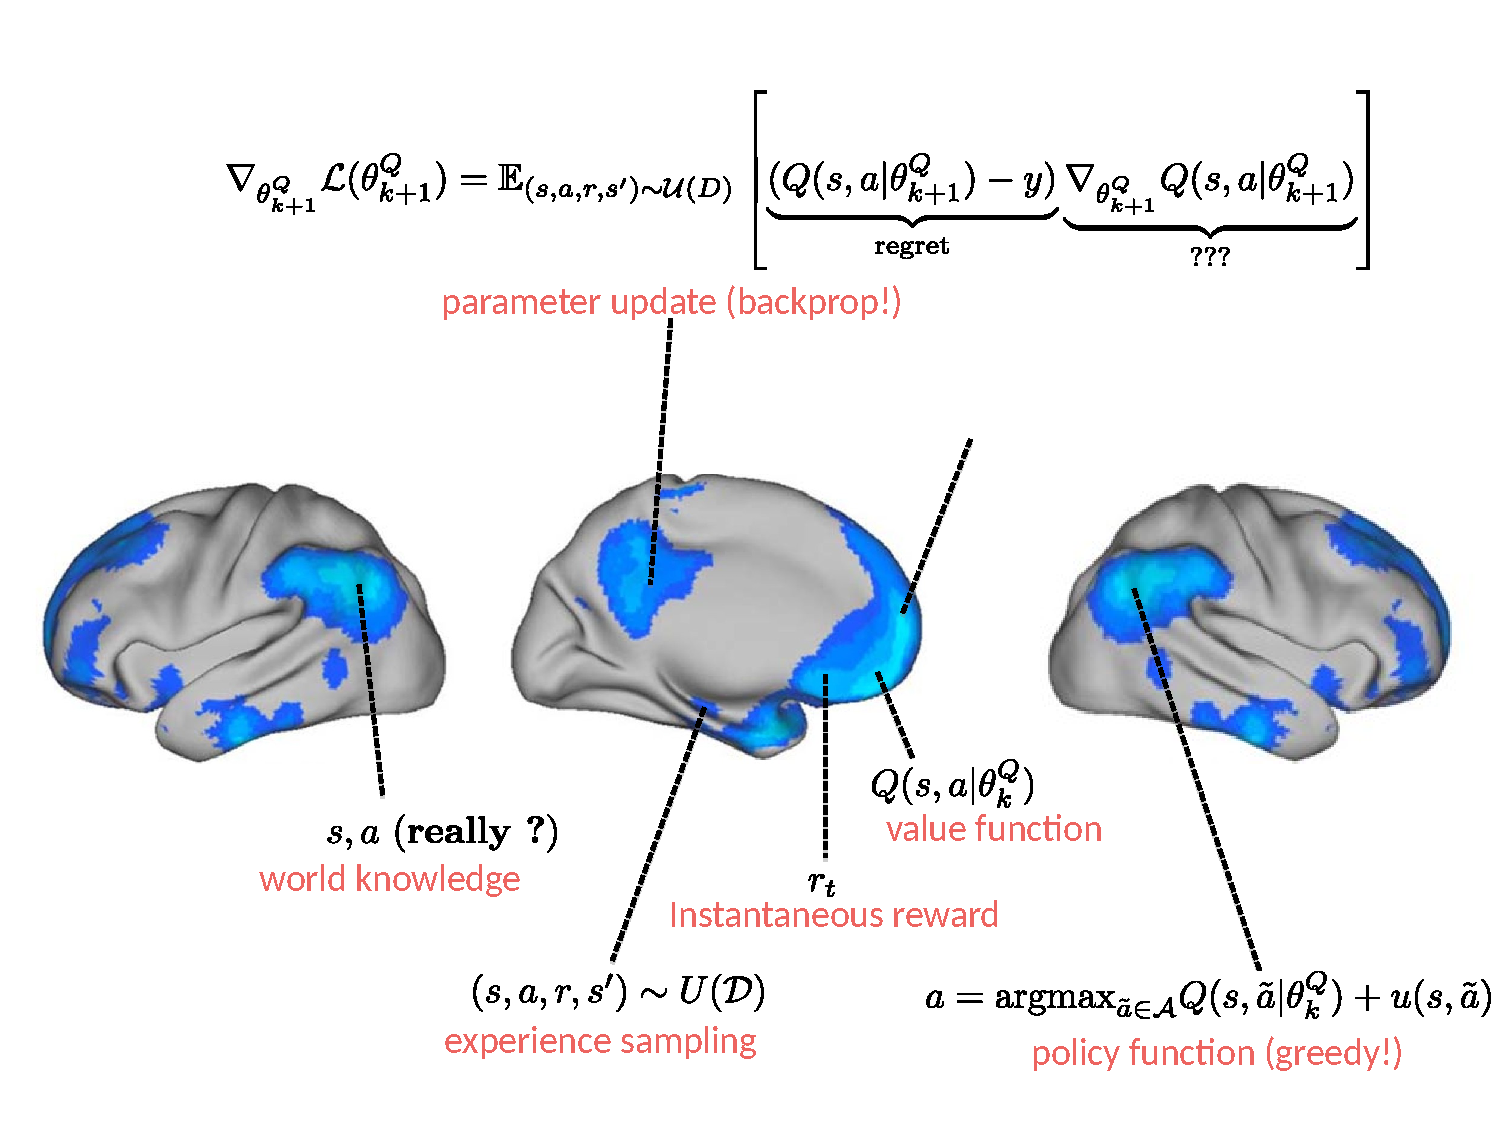
\includegraphics[width=.9\linewidth]{rl_process_chart.pdf}
  \caption{The DMN as an RL agent... \textbf{Please add a figure caption}}
  \label{fig:rl_process_chart}
\end{figure}
The DMN is today known to consistently increase in neural
  activity when humans engage in goal-directed behavior that are detached from
  current sensory environment \citep{kenet2003spontaneously, fiser2004small}
  and it was proposed to be situated at the top of the functional network hierarchies
  \citep{carhart2010default, margulies2016situating}.
  Its involvement in thinking about the past,
  the future, and hypothetical possibilities ties in with the implicit computation of
  action and state cascades as a function of what happened in the past.
  A policy represents the repertoire of possible actions
    on the world given a current state. It encodes the probabilites of
    choosing actions to be executed in a certain situation.
% Interactions between external and internal sources of
%   information are probably commonplace during perception \citep{gershman2010learning}
The DMN may subserve
  constant exploration of possible future actions and their
  cumulative reward outcomes. Implicit computation of future choices
  provides an explanation for the
  evolutionary emergence and practical usefulness of mind-wandering
  in humans.

The HC may provide perturbed action-transition-state-reward samples
  as batches of "imagined", "hypothesized", "recalled" experience.
  The small variations in these experience samplings allow searching
  a larger space of model parameters and possible experiences.
  Taken to its extreme, stochastic recombination of experience
  building blocks can further optimize the behavior of the RL agent
  by model learning from scenarios in the environment that the agent might
  only very rarely or never encounter.
  An explanation is thus offered for encountering seemingly familiar situations that
  a human has however never actually encountered (i.e., d\'{e}j\`{a} vu effect).
  While such a situation may not have been experienced in the physical world,
  the DMN may have already stochastically generated, evaluated, and adapted to
  such a randomly synthesized situation in the past.
  In the absence of environmental input and feedback
  (e.g., mind-wandering or sleep) pseudo-experiencing (i.e., emulating) possible
  future scenarios and action outcomes.
  Our approach thus acknowledges the unavoidable stochasticity of
  computation in neuronal processes \citep{faisal2008noise}.

  In our proposed model-free RL-based view, \textit{inference} in the human brain reduces to
  generalization of
  policy and value adaptations from sampled experiences to
  successful action choices and reward predictions in future states.
  As such,
  plasticity in the DMN arises naturally:
  If an agent behaving optimally in a given environment moves
  to novel, yet unexperienced environments, reward prediction errors will
  massively increase \textbf{Please complete sentence}.
  This will lead to adaptation of the policy until the system converges to a
  new steady-state of optimal action decisions in volatile environments.

% \paragraph*{Some notes:}
% \begin{itemize}
%   \item Actions are continuous, whilst states are continuous.
%   \item The brain does backprop (see Hinton's recent talk at Stanford)
%   \item model weights $\theta^Q$ should correspond to connections between neurons
% \item humm, looks like such a knowledge would simply translate into constraints on the DqN weights $\theta^Q$ (... at least, part of such knowledge)
%   ok, gotta think about the model-free / model-based reconsiliation
% \end{itemize}

\section{Relation to other models decision-making and optimal control for the brain}
\subsection{The free-energy principle and active inference}
% \subsubsection{The theory}
In Friston's free-energy principle (FEP) \citep{friston2010free,fristonAIorRL}, the brain is portrayed
as biomechanical inference engine which must minimize the long-term average of surprise.
Precursors of this theory can be traced back to \citep{dayan1995helmholtz} in which they introduced the so-called \textit{Helmholtz machine}, a hierarchical factorial \textit{directional deep belief-net (DBN)}. According to FEP's account, the goal of the brain is then to optimize over the generative model $G$: to iteratively
modify its internal representation $p_G(\z|\x)$ about objects in the world, their interactions and dynamics, etc., so as to minimize surprise when these representations are confronted with sensory input $\x$ during perception cycles. These is called the \textit{generative} model. FEP also postulates a dual model called the \textit{recognition} model,
which works in tandem with the generative model $p_R(\z|\x)$, to accomplish approximate inference. The recognition model dreams / fantasizes imaginary worlds $\z$ whilst the latter tries to generate sensations $\x$ which match these dreams!

Because surprisal is intractably difficult to optimize (since we would need to sum over all hidden causes of the sensations), FEP sets out to instead minimize an upper-bound thereupon, namely the \text{free-energy} $F_G^R(\x)$ given by

  \begin{equation}
    \begin{split}
      \text{generative surprise } &:= -\log(p_G(\x)) = F_G(\x) \\
      &=\underbrace{F^R_G(\x)}_{\text{accuracy}} - \underbrace{D_{KL}(P_R(.|\x) || P_G(.|\x))}_{\text{complexity}} \\
      &\le F^R_G(\x),
      \text{ with equality if }p_R(\z|\x) = p_G(\z|\x)\text{ for all } \z
    \end{split}
  \end{equation}

% \begin{figure}[!tb]
%   \centering
%   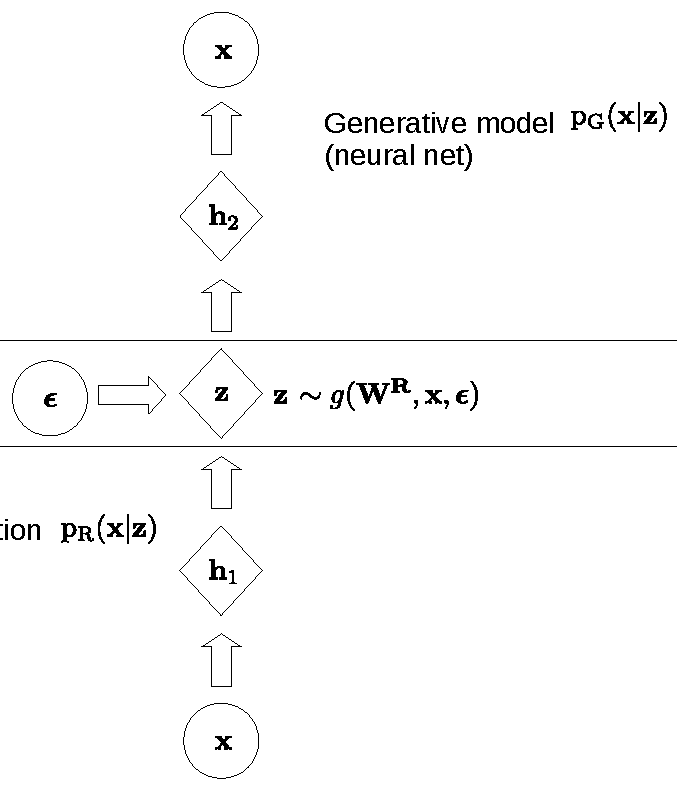
\includegraphics[width=.8\linewidth]{vae.pdf}
%   \caption{Variational autoencoders...}
%   \label{fig:vae}
% \end{figure}
The main algorithm for minimizing free-energy $F_G^R(\x)$ is the \textit{wake-sleep algorithm}.
\citep{dayan1995helmholtz}. As noted already in \citep{dayan1995helmholtz},
a crucial drawback of the wake-sleep algorithm is that it requires a concurrent models (generative and recogntiion), which together do not correspond to optimization of (a bound of) the marginal likelihood (because of the incorrect KL used therein, etc.). Thus the brain could not possible be running such a algorithm, not even in principle! To the rescue, we note that the recent theory of
\textit{variational auto-encoders (VAEs)} \citep{kingma2013auto} might provide an efficient alternative to the wake-sleep algorithm, as it overcomes the technical limits of the former, by using a reparametrization trick. For instance, unlike the wake-sleep algorithm for minimizing free-energy, VAEs can be efficiently trained via back-propagation of learning errors.

\subsubsection{Comparison to our proposed theory}
On the surface, a common point between the FEP and our proposed RL-based framework
  is placing the minimization of a surprise signal at the core of brain function.
  Indeed in RL, surprise minimization is subsumed  by accurate prediction of
  rewarding outcomes in the future. A ``free-energy'' agent is barely a biomechanical machine which has the tendency to resist undesired / harmful phase-transitions.
  \citep{friston2010free,fristonAIorRL,ortega2013thermodynamics}. Such a theory cannot by itself,
  explain the emergence of strategic behavior inherent in humans (e.g.,  cite dark-room experiment).

% Friston's critic of RL \citep{fristonAIorRL} (he proposes ``active inference''): "This equation (equation 18) comes from the theory of dynamic programming,
% pioneered in the 1950s by Richard Bellman and colleagues [2]. To
% optimise control a~pð Þ x~ under this formulation, we have to: (i)
% assume the hidden states are available to the agent and (ii) solve
% Equation 18 for the value-function. Solving for the value-function
% is a non-trivial problem and usually involves backwards induction
% or some approximation scheme like reinforcement learning [4–6].
% The free-energy formulation circumvents these problems by
% prescribing the policy in terms of free-energy, which encodes
% optimal control (Equation 6)"

% The following critics can be made:
% \begin{itemize}
%   \item
%     As noted by Dayan et al. (\textit{Variants of Helmholtz machines}), the inter-neuronal intra-layer independence assumption which is at the center of the HM becomes severely problematic as it is agnostic to the known organization of cortical layers...
%   \item A drawback of the wake-sleep algorithm is that it requires a concurrent models (generative and recognitiion), which together do not correspond to optimization of (a bound of) the marginal likelihood (because of the incorrect KL used therein, etc.).
%   \item Also, note that the wake-sleep algorithm doesn't do backprop! This is due to
%     technical difficulty in getting derivatives of loss function w.r.t
%     recognition weights $\W^R$).
%   \item This difficulty was removed in the 2010s by \citep{kingma2013auto}, an other groups, via a ``reparametrization trick''.
%   \end{itemize}

\textbf{XXX: add tons of more examples and connnections}
\textbf{XXX: integrate aspects from section "ThE MARkOv DECISION PROBLEM" in Dayan and Daw}
\textbf{XXX: integrate aspects from WakeNsleep by Hinton}
\textbf{XXX: integrate aspects from Friston2014(Dropbox) on active inference}
\textbf{XXX: integrate aspects from Sutton/Barto book chapter}

\subsection{Predictive Coding Hypothesis}
The predictive coding framework
\citep{clark2013whatever, friston2008hierarchical}
is a frequently evoked idea related to the default mode function
\citep{bar2007}.
According to this cognitive account,
cortical responses emerge from continuous functional interaction between
higher and lower levels of the neural processing hierarchy.
This dynamic intercourse enables inference on the world by reconciling
gaps between fresh sensory input and stored prior information.
Feed-forward sensory experience is constantly calibrated by
top-down modulation at various hierarchical processing levels.
In fact, axonal
back projections probably outnumber by far the input projection
existing in the brain \citep{salin1995corticocortical}.
This can explain the constructive, generative nature of sensory perception
\citep{friston2010free} and
why motor action is intimately related to sensory expectations
\citep{wolpert1995internal, kording2004bayesian}.
At each stage of neural processing,
an internally generated prediction of the sensory input is
directly compared against the actual input from the environment.
A prediction error at one of the processing levels,
i.e. the difference between sensory input
and internally predicted sensation,
incurs plasticity changes of neuronal back projections (i.e., model parameters)
for gradually improved future prediction of the environment.
Contextual integration is hence maintained by top-down modulation of sensorimotor
processing by a-priori information about the environment.
The generative model of how perceived sensory events arise in the
world would be incorporated into
the current neuronal wiring.
Indeed,
This process permits updates of the internal model of the environment
to best fit the constant influx of sensory examples.


\begin{itemize}
  \item Both the predictive coding account and POMDPs
  are process theories backed up by plausible
  neurobiological evidence that
  view the brain as a ``statistical organ''
  generalizing from the past to new experiences.
  \item Both provide a parsimonious explanation why the
  human brain decreases processing load devoted to incoming information
  when the environment is predictable and allocate increased
  attentional resources when novel stimuli are encountered.
  Similarly, both propose explanations why
  predicting the future is inherently
  linked to information from the past.
  \item Sensory experience is a generative process from both views.
  In predictive coding, sensory perception of the external world
  is a generative experience due to modulatory top down experience at
  various hierarchical levels of sensory input processing.
  In our RL view, the (partially observed)
  environmental model is incorporated in the POMDP,
  \textit{which can be fully recovered based on the last
  state alone}.
  \item Both naturally expose a mechanisms of brain plasticity in that
  neuronal wiring gets increasingly adapted
  when faced by unprecedented environmental
  challenges.
  \item The hierarchical aspects from predictive coding
  is re-expressed in POMDPs in form of
  nested prediction of probable upcoming actions and rewards.
  \item Both model the consequences of action. In RL, the horizon of that
  look into the future is explicitly manifested in the $\gamma$ parameter
  in the Bellman equation, but not
  explicitly modeled in the PC account that
  tends to emphasize prediction about the
  immediate future.
  \item \suggestremove{Mismatch negativity of PC is immanent in reward prediction error
  by the difference between actually predicted reward of an action given
  a state and the reward predicted by non-linear regression with graded
  discounting of future rewards.}
  \item Adapting the neuronal connections for improved top-down modulation
  takes the concrete form of gradient computation
  \textit{and back-propagation} in MDPs and RL,
  although the neurobiological plausibility of
  the back-propagation procedure is controversal
  \citep{goodfellow2016deep}.
  \item In sum,
  the MDP account may serve as a concrete conceptualization of the PC account
  in cognitive neuroscience. MPDs have the advantage of exposing an explicit
  mechanism of the horizon of future considerations or
  how the internal model of the world gets updated,
  and collapses sensory input processing and action output preparation.
  %
  As such, our MDP account of DMN function can parsimoneously explain
  prediction coding hypothesis.
\end{itemize}


\subsection{Semantic Hypothesis}
Another frequently proposed cognitive account of DMN function revolves
around forming logical associations and analogies between
the current experience and
the conceptual knowledge derived from past experiences
\citep{bar2007proactive, binder1999conceptual}.
Analogies might naturally tie incoming novel sensory stimuli to
explicit world knowledge (i.e., semantics) extractable from the environment
\citep{bar2009proactive}.
In this way, the encoding of complex environments could be facilitated
by relative similarity associations between states.
%
Going much beyond human language ifself,
semantic building blocks provide the basis to
mentally envision non-existent scenarios
that would improve optimal behavior in the environment
by simulating future events.
Such cognitive processes can afford
the internal generation of necessary information
that is not presented in the surrounding environment
by recombining building blocks of
concept knowledge and episodic memories
\citep{hassabis2009construction}.
Indeed, in aging humans, remembering the past and imaging the future
equally decreased in the level of detail and are associated with
concurrent deficits in forming and integrating relationships between
items \citep{addis2008age, spreng2006temporal}.
Further,
a constructive account explains the reciprocal relationship
between an egocentric first person perspective and
an allocentric bird’s eye perspective immersed in
self-reflection, social knowledge, and autobiographical memories.
%
Cognitive aspects of egocentric-allocentric switching
are also closely related to episodic memory, language, problem solving,
planning, estimating other people's thoughts, and spatial navigation
as these necessitate abstract world knowledge and abstract assocations
for binding the constituent elements in mental scene construction
\citep{schacter2007remembering}.
These scene generation processes could contribute to interpreting the
present and foretelling the future.
This view is for instance supported by evidence in animals that
could learn a \textit{cognitive map of the environment},
even without reward incentives, and exploit it later
for other means \citep{tolman1948cognitive}.



\begin{itemize}
  \item Both the semantic hypothesis and MDPs expose mechanisms of
  how alternative decision trees could be mentally explored.
  \item In both semantic hypothesis and MDPs,
  there is no evidence to indicate that predictions of various
  levels of complexity, abstraction, timescale and purpose
  use mechanisms that are qualitatively different. This concurs with
  DMN activity increases across time, space, and content domains
  demonstrated in many neuroimaging studies. The semantic hypothesis
  and RL account provide explanations why hippocampus lesion does
  not only impair retrieving memories, but also hypothetical and future
  thinking \citep{hassabis2007patients}.
  \item The notion of semantic or knowledge association is
  incorporated into the MDP as the Markov property,
  that is, the current state directly results from the
  agent's history of states and actions. The learned
  value matrix and action transition schedules drive
  stimulus processing and action choice in the present.
  \item Mental scene construction has been proposed by some authors
  \citep{buckner2007self} to imply a distinction between
    environmental perception and internally generated mind-wandering\footnote{
      \textbf{XXX Elvis: This is more than just a footnote. Make this part of the paper
      and factorize the lot. Also you probably need a citation here!!!}
  ``A computational model of how such a process might be structured
  is far from being defined, but it will probably require a form of
  regulation by which perception of the current world is suppressed
  while simulation of possible alternatives are constructed,
  followed by a return to perception of the present.''\citep{buckner2007self}}.
  The MDPs naturally integrate the former egocentric
  (more related to current action, state and reward) and the later
  allocentric (more related to past and future actions, states, and rewards)
  angles on the world in a same optimization problem.
  \item The semantic account of DMN function does not offer
  a mechanistic explanation how explicit world knowledge and semantic analogies thereof
  lead to prediction of future actions and states.
  \item In contrast to existing accounts on semantics and
  mental scene construction, the random and creative aspects of DMN function
  are explained in MDPs by the advantages of stochastic optimization.
  \item The semantic hypothesis does not explain why memory recall
  for scene construction in humans is typically fragmentary and noisy
  instead of accurate and reliable.
  Yet, the MDP framework provides an algorithmic explanation in that
  stochasticity of the parameter space explored
  by the Monte Carlo solvers achieves better fine-tuning of the
  action policies and estimation of expected reward outcomes.
  That is, the purposeful stochasticity of policy and value estimation
  in MDPs provides a candidate explanation for why humans
  have evolved imperfect noisy memories
  as the more advantageous adaptation.
  \item While both semantic and MDP account propose memory-based internally
  generated information for probabilistic mental models of action outcomes,
  only MDPs render explicit the grounds on which the final action is
  eventually chosen (i.e., the estimated cumulative reward).
  \item In sum, episodic scene construction according to the semantic
  hypothesis is lacking an explicit time and incentive model;
  neither does it explain how randomness of human mental experience
  can be beneficial.
\end{itemize}



\subsection{Sentinel Hypothesis}
Processing self-relevant information was perhaps the first
cognitive account that was proposed for the DMN \citep{gusnard2001medial}.
Since then,
different investigators have speculated that neural activity in the DMN
may reflect the brain’s relentless tracking of
relevance in the environment
as an advantageous evolutionary adaptation.
According to this cognitive account, the brain's baseline realizes
a ``radar'' function to
detect subjectively salient and unexpected events that
are the most important for unfolding behavior,
including resources,
the securing of mates, and protection.
%
In fact,
environmental stimuli important for humans are frequently of
social nature. This is probably unsurprising
given that a key property of the human species is
the complexity of their social systems
\citep{tomasello2009cultural}.
More specifically,
according to the ``social brain hypothesis'',
the human brain did not evolve to solve problems of the
physical environment, but to form and maintain increasingly complex
social systems to solve ecological problems by means of social relationships
\citep{whiten1988machiavellian}.
Highly efficient neurobiological processing of social cues is exemplified by
facial judgments being routinely processed in less than 100 ms
\citep{bar2006very}.
Our human ancestors were probably among the few organisms that
were more likely to be killed by members of their own species
rather than predators from another species.
Being able to detect the intention and upcoming actions of conspecifics
turned into a decisive evolutionary advantage
\citep{frith2010social}.
%
This may explain why social topics amount to roughly
two thirds of human everyday communication \citep{dunbar1997human}
and
why mind-wandering and dreams
are so rich in stories about people and
the complex relationships between them
\citep{schilbach2008minds}.


\textbf{XXX Elvis: Your focus in this subsection ought to be on the SC itself not POMPDs. -> agree I will fix it later.}
 \begin{itemize}
    \item Processing social information has been proposed to underlie the
    physiological baseline of human brain function
    \citep{schilbach2008minds}. This was later challenged by observing
    analogues of the DMN in monkeys \citep{mantini2011default}
    and rats \citep{lu2012rat}, with
    supposedly less advanced social capacities.
    The MDPs parsimoneously explain the dominance of social content in
    human mental scenes by their extremely high relevance to humans
    reflected by high values for social information in the value matrix
    \citep{baker2009action}.
    \item How can a same neurobiological circuit be equally important
    for baseline house-keeping functions and specific task performance?
    Our computational account can explain why the DMN is implicated
    in both a goal-directed task and an idlying rest cognitive set,
    if environmental relevance is processed, manipulated, and retained
    also as a baseline function of human mental activity.
    In tasks, the policy and value matrices are updated to optimize short-term action,
    whereas, at rest, these parameter updates may
    improve especially mid- and long-term action.
    \item The sentinel account does not provide a formal mechanisms of
    how attention and memory resources are exactly reallocated when
    encountering a salient environmental stimulus. \textbf{XXX remove the next sentence. Danilo: can you help me to correct the sentence instead.
    There appears to be a cool link between cognition and formal theory
    here. Elvis: I'd've helped you correct it but, i don't quite understand what you wanted to say. For ex, note that $\sum_{a \in \mathcal A}\pi(a|s) = 1$ for any state $s$,
  and so it doesn't quite make sense to talk about weighting things with ``$\sum_{a \in \mathcal A}\pi(a|s)$''.}
    In contrast,
    the Bellman recursion is weighted at each step by
    $\sum_{a \in A}\pi(a|s)$. This factor weighs which action cascades
    are recursively explored by the agent and which decision trees are neglected.
    This directly implies allocation of attention and computational load.
    \item In sum,
    MDPs imply a ``radar'' function of monitoring the environment for salient information
    in general and explain social thinking as a physiological brain baseline
    as an important special case, without excluding other topics
    contemplated in continuous mental activity.
 \end{itemize}



\section{Conclusion}
What brain function could be important enough
for the existence and survival of the human species
to warrant constant, high energy costs?
MDPs provide an attractive
process model how the human association cortex
might implement supra-modal representation and control of the environment to
optimize the organism's fate.
% by obtaining reward and avoiding pain.
This idealized process model explains
a number of previous experimental observations in the
DMN by a simple but non-trivial mechanism.
%
From the computational view of a Markovian sequential decision process,
behavior unfolds by integrating happened past events
and possible future events to guide action choice in the present context.
This functional account is more compatible with the DMN's
poorly understood involvement across
autobiographical memory retrieval, problem solving,
abstract reasoning based on internally generated scenes, social cognition,
as well as delay discounting and self-related prospection.
MDPs provide a mathematical formalism how
optimal substructure in the environment can be recursively exploited
when confronted with complicated decisions.
Improvement of the internal world model
by injecting stochasticity in the recall of past
actions and outcomes may explain why
very accurate memories have been disfavored in human evolution
and why human creativity might be adaptive.
%
In principle,
neuroscientific experiments can be designed that operationalize
the set of action, value, and state variables that determine
the behavior of intelligent RL systems.
The proposed machine-learning perspective
on DMN biology is hence not only practically computable but
also neuroscientifically falsifiable.
At the least, we propose an alternative vocabulary to
describe and interpret experimental findings in neuroscience studies
on the DMN.
%
Ultimately,
the DMN can be viewed as a functional integrator
from the relatively recent events to anticipated upcoming events
in order to constantly improve present action in our dynamic world.



\paragraph{Acknowledgment}
% {\small The research leading to these results has received funding from the
% European Union Seventh Framework Programme (FP7/2007-2013)
% under grant agreement no. 604102 (Human Brain Project).
% Further support was received from
% the German National Academic Foundation (D.B.).
% }


\small
% \bibliographystyle{splncs03}
% \bibliographystyle{natbib}
\bibliographystyle{plainnat}
\bibliography{refs}

\appendix
\section{Free-energy principles!}
The so-called free-energy principle in its present form (including notions like ``generative density'', ``recognition density'', etc.) can be traced back to works of Dayan \& Hinton \citep{dayan1995helmholtz} in which they introduced the so-called \textit{Helmholtz machine}, a hierarchical factorial directional deep belief-net (DBN).
In this subsection, we will develop from first-principles, the bare-bones minimalistic ideas needed to build a free-energy principle for general decision-making. This ideas were first developed by Hinton et al. in the early 90s in building their Helmholtz machine. Theories like Friston's free-energy principle and active-inference will then emerge as particular instances of this general framework, with particular design choises. For instance, the Friston theory axiomatizes that the brain uses a (problematic, as it implicitly assumes that posterior of each hidden unit is factorial) wake-sleep algorithm to train the underlying Helmholtz machine, etc.

% \begin{mdframed}
%   Though our presentation of free-energy principles is thermodynamic in flavor, a completely equivalent
%   information-theoretic formulation is of course possible, simply by exploiting the information-theoretic interpretation of entropy.
% \end{mdframed}

\subsection{Helmholtz free-energy and the generative model}
\begin{table}[H]
  \begin{tabular}{p{2cm}|p{11cm}}
         \hline
         \textbf{symbol}    & \textbf{description}  \\ \hline
         $\langle X\rangle_p$ & Expectation (a.k.a average, a.k.a mean value) of the
         random quantity $X$ w.r.t to the probability density $p$, formally defined by $\langle E\rangle_p := \sum_{z}p(z)X(z)$.\\ \hline
         $\mathcal H(p)$ & Information-theoretic entropy of a probability density $p$, formally defined by $\mathcal H(p) := -\sum_{z}p(z)\log(p(z))$,
          with the usual convention $0 \log(0) := 0$.\\ \hline
         $D_{KL}(q||p)$ & The Kullback-Leibler divergence between the probability densities $q$ and $p$ respectively, formally defined by $D_{KL}(q||p) := \sum_{z}q(z)\log(q(z)/p(z))$.\\ \hline
             $\x$ & Observations. In Friston's free-energy principle this has a decomposition in to two terms: the brain's internal state $b$ and sensory inputs $s$, i.e $\x = (s, b).$ \\ \hline
             $\z$ & Hidden variables. This should be understood as the unobservable states of the external environment (to which the brain is trying to adapt by learning).\\ \hline
             $p_G(.|\x)$ & Generative density for ...\\ \hline
         $p_R(.|\x)$ & Recognition density for ... Does some kind of predictive coding (?).\\ \hline
         $F_G(\x)$ & Helmholtz free-energy for a model $p_G$ of generating the observation $\x$. This measures the surprise incured upon observing $\x$ generated by the model $G$.\\ \hline
         $F^R_G(\x)$ & Variational Helmholtz free-energy from model $G$
          to $R$.  Note that $F^G_G = F_G$.\\ \hline
  \end{tabular}
  \caption{Table of notations.}
\end{table}
Our starting point will be to build an approximation $p_G$ for the true density $p$ of the observations, so that this approximate density corresponds to the partition function of thermodynamic system. So,
\begin{eqnarray}
  \begin{split}
    \text{generative surprise } &= -\log(p_G(\x)) = -\log(p_G(\x)) \times 1 = -\log(P_G(\x))\sum_{\z}p_G(\z |\x)\\
    &= -\sum_{\z}p_G(\z, \x)\log(p_G(\x))
    =-\sum_{\z}p_G(\z |\x)\log(p_G(\z, \x)/p_G(\z|\x))\\
    &= \sum_{\z}p_G(\z |\x)\log(p_G(\z|\x))-\sum_{\z}p_G(\z |\x)\log  (p_G(\z, \x))\\
    &= -\langle \log  (p_G(., \x)) \rangle_{p_G(. |\x)} - \mathcal H(p_G(. |\x))\\
    &= \langle E_G(., \x) \rangle_{p_G(. |\x)} - \mathcal H(p_G(. |\x))
  \end{split}
  \label{eq:helm}
\end{eqnarray}
where $E_G(\z, \x)$ is the energy at \textit{macrostate} $\z$ of a fictive thermodynamic system defined by setting
\begin{equation}
  E_G(\z, \x) := -\log(p_G(\z, \x)),
  \label{eq:gibbs}
\end{equation}
%% In the above, the variable $\z$ is a hidden variable, and can / should be interpreted as the unobservable state of the external world.
The last quantity in \eqref{eq:helm} is nothing but \textit{Helmholtz free-energy} (at unit temperature!), defined formally by
\begin{equation}
  F_G(\x) := \langle E_G(., \x) \rangle_{p_G(. |\x)} - \mathcal H(p_G(. |\x)).
\end{equation}
%% , modelled as the physical system for which $p_G(\z|\x)$ dictates the occupation probabilities of macrostates $\z$
Thus,
\begin{fact}
  Generative surprise and generative Helmholtz free-energy are different views on exactly the same object.
\end{fact}

The goal of the brain is then to optimize over the generative model $G$: to iteratively or analytically modify the generative density $p_G(.|\x)$, so as to minimize surprise. It turns out that a direct attempt to attack this optimization problem by gradient descent on the free-energy $F_G(\x)$ is furtile: the parameter update steps are not ``very clean'', and require rather cumbersome and heavy computations. A workaround is then to introduce a second density $p_R(.|\x)$ called a \textit{recognition} density to work in tandem with the generative density $p_G(.|\x)$, as a trick for doing approximate inference. The former dreams / fantacizes whilst the latter tries to generate sensations which match these dreams! This primal-dual idea, first proposed in Hinton et al. 1995, is at the heart of the general free-energy principle that we will introduce shortly.

\subsection{Variational Helmholtz free-energy and the bottom-up recognition sub-model}
In this subsection, we will present an insightful upper bound for the generative surprise (i.e generate Helmholtz free-energy), called the \textit{variational} (Helmholtz) free-energy. As an avant-gout of what is to come shorty, let's just note that the well-known \textit{free-energy principle} is simply a workaround whereby the minimization surprise (intractable) is replaced with the  minimization a carefully chosen upper bound thereof.

Invoking \eqref{eq:gibbs} and applying Bayes rule, we get the Gibbs
distribution
\begin{equation}
  p_G(\z|\x) = \frac{p_G(\z|\x)}{p_G(\x)} = \frac{\exp(-E_G(\z, \x))}{Z_G(\x)} = \frac{\exp(-E_G(\z, \x))}{Z_G(\x)},
\end{equation}
where $Z_G(\x) := \log(p_G(\x)) = \sum_{\z'}\exp(-E_G(\z',\x))$, the normalizing \textit{partition function} for the model \ref{eq:gibbs}.
Whence, for any macrostate $\z$, we have $p_G(\x) = Z_G(\x) = \exp(-E_G(\z, \x)) / p_G(\z|\x)$, and so it holds that
\begin{equation}
F_G(\x)\overset{\eqref{eq:helm}}{=} -\log(p_G(\x)) = -\log(Z_G(\x)) = E_G(\z, \x) + \log(p_G(\z|\x)).
\end{equation}
Now, in the above equation, the LHS only depends on the generative model $G$ and the data point $\x$:
it doesn't depend on the hidden variable $\z$, etc. So, taking expectations w.r.t an arbitrary
density\footnote{conditioning in $P_R(.|\x)$ is because this density is selected from a world in which the sensory inputs and internal brain
  state vector $\x$ is assumed already observed.} $p_R(.|\x)$ yields
\begin{equation}
  \begin{split}
    F_G(\x) &= -\log(Z_G(\x)) = \langle E_G(., \x)\rangle_{P_R(.|\x)} + \sum_{\z}p_R(\z|\x)\log(p_G(\z|\x))\\
    &= \langle E_G(., \x)\rangle_{P_R(.|\x)} - \mathcal H(p_R(.|\x)) - \sum_{\z}p_R(\z|\x)\log(p_R(\z|\x)/p_G(\z|\x))\\
    &= F^R_G(\x) - D_{KL}(P_R(.|\x) || P_G(.|\x)),
  \end{split}
  \label{eq:fe}
\end{equation}
where $F^R_G(\x)$ is the \textit{variational} Helmholtz free-energy from $R$ to $G$ defined by
\begin{equation}
  F^R_G(\x) := \langle E_G(., \x)\rangle_{P_R(.|\x)} - \mathcal H(p_R(.|\x))
\end{equation}
and $D_{KL}(P_R(.|\x) || P_G(.|\x))$ is the Kullback-Leibler divergence between the $p_R(.|\x)$ and the generative density $p_G(.|\x)$. Note that $F^G_G = F_G$.

\subsection{A general free-energy principle}
We can resume the situation as follows\footnote{Where we have used the fact that KL divergence is always nonnegative.}:
\begin{mdframed}
\begin{equation}
  \begin{split}
    \text{generative surprise } &:= -\log(p_G(\x)) = F_G(\x) \\
    &=\underbrace{F^R_G(\x)}_{\text{accuracy}} - \underbrace{D_{KL}(P_R(.|\x) || P_G(.|\x))}_{\text{complexity}} \\
    &\le F^R_G(\x),
    \text{ with equality if }p_R(\z|\x) = p_G(\z|\x)\text{ for all } \z
    \end{split}
\end{equation}
\end{mdframed}
%% In fact, we have the following theorem
%% \begin{theorem}
%%   It holds that
%%   $$
%%   \text{Minimal generative surprise = minimal (Helmholtz) variational free-energy},$$
%%   i.e
%%   \begin{equation}
%%     \min_{G}F_G(\x) = \min_{G,R}F^R_G(\x)
%%     \end{equation}
%% \end{theorem}

\subsection{Helmholtz machines and the wake-sleep algorithm}
% \begin{mdframed}
  \textbf{Assumption:} In both generative and recognition components of the network, there is conditional independence of  neurons in the same layer, given the data (i.e input from lower more primitive layers). Precisely
$$
p_G(\z^{(l)}|\x) = \Pi_{k=1}^{h_l}p_G(\z_k^{(l)} | \x),\hspace{1cm}
p_R(\z^{(l)}|\x) = \Pi_{k=1}^{h_l}p_R(\z_k^{(l)} |\x)
$$
% \end{mdframed}

\subsection{Friston's active-inference and agency}
\label{sec:friston}
This is nothing but an application of the Dayan's wake-sleep algorithm for training a Helmholtz machine model of the brain...

The following critics can be made:
\begin{itemize}
  \item
    As noted by Dayan et al. (\textit{Variants of Helmholtz machines}), the inter-neuronal intra-layer independence assumption which is at the center of the HM becomes severely problematic as it is agnostic to the known organization of cortical layers...
  \item A drawback of the wake-sleep algorithm is that it requires a concurrent models (generative and recognitiion), which together do not correspond to optimization of (a bound of) the marginal likelihood (because of the incorrect KL used therein, etc.).
  \item Also, note that the wake-sleep algorithm doesn't do backprop! This is due to
    technical difficulty in getting derivatives of loss function w.r.t
    recognition weights $\W^R$).
  \item This difficulty was removed in the 2010s by \citep{kingma2013auto}, an other groups, via a ``reparametrization trick''.
    \end{itemize}


\subsection{Minimizing free-energy via backprop: variational auto-encoders}

% \subsection{Free-energy minimization via variational auto-encoders}
\label{sec:vae}
Here, we present a way to alleviate some conceptual and computational issues with the
free-energy framework presented thus far, by using the recent \textit{variational auto-encoder} (VAE) theory \citep{kingma2013auto}. Define the data-dependent
auxiliary random function
\begin{eqnarray}
  f_{G,R}(., \x) :\z \mapsto \log(p_G(\z,\x)) - \log(p_R(\z|\x)).
\end{eqnarray}
Then we can rewrite the
variational free-energy as
\begin{eqnarray*}
  \begin{split}
    F_G^R(\x) &:= \langle E_G(., \x) \rangle_{p_R(. |\x)} - \mathcal H(p_R(. |\x)) = \langle E_G(., \x) + \log(p_R(.|\x))\rangle_{P_R(.|\x)}\\
    &=\langle -\log(p_G(.,\x)) + \log(p_R(.|\x))\rangle_{P_R(.|\x)}\\
    &= -\langle f_{G,R}\rangle_{P_R(.|\x)} \approx -\frac{1}{M}\sum_{m=1}^Mf_{G,R}(\z^{(m)}), \text{ with }\z^{(1)},\ldots,\z^{(M)} \sim p_R(.|\x), \text{ and }M \rightarrow \infty.
    \end{split}
\end{eqnarray*}

\begin{mdframed}
  \textbf{Problem:} How do we sample from the recognition density $p_R(.|\x)$ in such a way that the sampling process is differentiable w.r.t the weights of the recognition network $\W^R$ ?
\end{mdframed}

\begin{figure}[!tb]
  \centering
  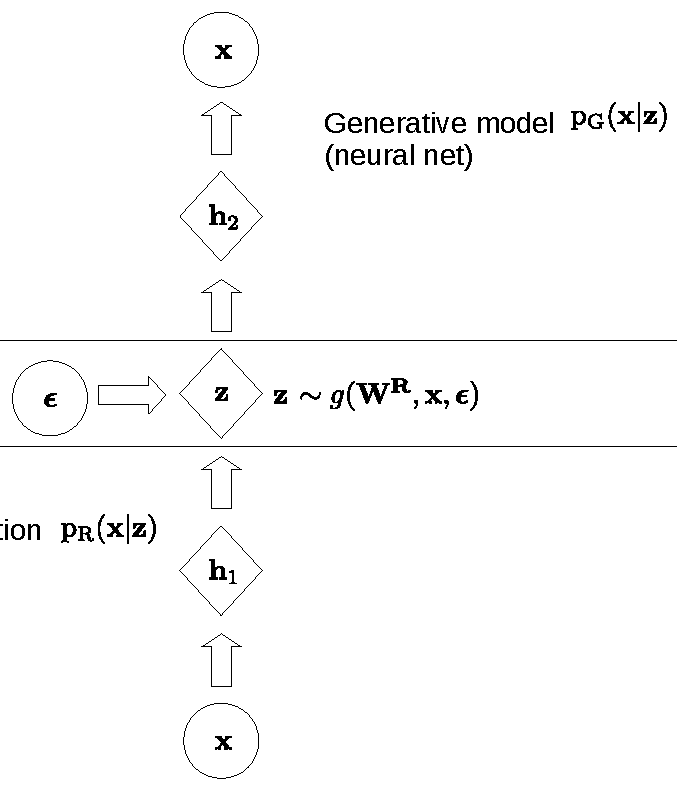
\includegraphics[width=.8\linewidth]{vae.pdf}
  \caption{Variational autoencoders...}
  \label{fig:vae}
\end{figure}

\paragraph{Solution: The reparametrization trick.}
\begin{itemize}
\item Choose $\epsilon \sim p_{\text{noise}}$ (noise distribution, independent of $\W^R$!)
\item Set $\z = g(\W^{R}, \x, \epsilon)$, where $g$ is an appropriate class $\mathcal C^1$ function
  \begin{itemize}
  \item results in a sample $\z \sim p_R(.|\x)$, from the correct
    posterior
    \end{itemize}
\end{itemize}
The mapping $g$ should be taught of as a ``blurring'' function which produces noisy versions $\z$,
called \textit{sensations}, of the true world state $\x$.
The result is a scheme for training DBNs via good-old backprop!
Refer to Fig. \ref{fig:vae}. Some examples of the reparametrization trick for a number of
choices of the posterior distribution are given in Tab. \ref{tab:rptrick}.

\begin{table}[H]
  \begin{tabular}{p{1.7cm}|p{1.5cm}|p{1.9cm}|p{2.1cm}|p{5cm}}
         \hline
         Posterior & $p_R(.|\x)$ & noise & $g(\W^R,\x,\epsilon)$ & Also \\ \hline
         Normal & $\mathcal N(\mu,\sigma)$ & $\epsilon \sim \mathcal N(0, 1)$ & $\mu + \sigma \odot \epsilon$ & Location-scale family: Laplace, Elliptical,
         Student’s t, Logistic, Uniform, Triangular, \ldots \\ \hline
         Exponential & $\mathcal \exp(\lambda)$ & $\epsilon \sim \mathcal U([0, 1))$ & $-\log(1-\epsilon)/\lambda$ & Invertible CDF: Cauchy, Logistic, Rayleigh, Pareta, Weibull, Reciprocal, Gompert, Gumbel, Erlan, ... \\ \hline
         Other & $\log\mathcal N(\mu,\sigma)$ & $\epsilon \sim \mathcal N(0, 1)$ & $\exp(\mu + \sigma \odot \epsilon)$ & Gamma, Dirichlet, Beta, Chi-squared, F, ... \\ \hline
  \end{tabular}
  \caption{Reparametrization trick \citep{kingma2013auto} for a variety of models.}
  \label{tab:rptrick}
\end{table}

%% For fixed $p_G(.|\x)$, the optimal choice for $p_R(.|\x)$ is given analytically by
%% \begin{equation}
%%   p_R(\z|\x) \propto p_G(\z|\x)\exp(-\Delta E_{G \rightarrow R}(\z, \x)).
%% \end{equation}

%% \subsection{A thermodynamic model for bounded rationality, aka robust
%%   optimality}
%% \begin{itemize}
%%   \item Recall that an agent is said to have \textit{bounded rationality} if they must take into account the cost of finding solutions to problems, and not just the utility of the final state.
%%   \item For example, consider an agent that must operate under a limited lifetime and/or computation cost.
%%   \item This is in contrast to agents with \textit{unbounded rationality} considered in classical game theory.
%%     \end{itemize}
%% The material presented is a revisit of \citep{braun2011path}. See also \citep{ortega2013thermodynamics}
%% \paragraph{Utility functions and conjugate pairs.}
%%   Let $(\Omega, \mathcal F, P)$ be a probablity space. A function $U: \mathcal F \rightarrow \mathbb R$ is said to be a \textit{utility function} for this space if the conditional utility $U(A|B) := U(A \cap B) - U(B)$ has the following propertites:
%%   \begin{itemize}
%%   \item additivity: $U(A_1 \cap A_2 | B) = U(A_1|B) + U(A_2|B)$, for all events $A_1, A_2, B \in \mathcal F$.
%%   \item statistic: there exists a function $f_{U} :\mathbb R_+ \rightarrow \mathbb R$ such that $U(A|B) = f(P(A|B))$, for all events
%%     $A,B \in \mathcal F$.
%%   \item monotonicity: $f_{U}$ is strictly increasing.
%%     \end{itemize}

%% \begin{theorem}
%%   The only functions $f: \mathbb R_+ \rightarrow \mathbb R$ which is such that $U(A|B) \equiv f(P(A|B))$ any probability space $(\Omega, \mathcal F, P)$ and utility function $U$ thereupon are of the form
%%   \begin{equation}
%%     f = \alpha \log(.),
%%     \label{eq:boltzmann}
%%   \end{equation}
%%   where $\alpha > 0$.
%% \end{theorem}

%% \textbf{XXX: equation \eqref{eq:boltzmann} above looks like Boltzmann's formula (on his gravestone...)!}

%% Such $U$ and $P$ are said to form a \textit{conjugate pair} at temperature $\alpha$.


%% \paragraph{Example.}
%% Given a utility function $U$ on a probability space $(\Omega, \mathcal F, *)$, the \textit{Gibbs measure} at temperature $\alpha > 0$ and energy levels $(-U(\omega))_{\omega \in \Omega}$ is defined to be the probability measure (on thesame measurable space)
%%   \begin{equation}
%%     P(\omega) = \frac{1}{Z_{U}(\alpha)}\exp\left(\frac{1}{\alpha}U(\omega)\right), \; \forall \omega \in \Omega,
%%   \end{equation}
%%   where

%%   \begin{equation}
%%     Z_{U}(\alpha) := \sum_{\omega \in \Omega}\exp\left(\frac{1}{\alpha}U(\omega)\right)
%%   \end{equation}
%%   is a normalization constant called the \textit{partition function} of $U$.
%%   It's not hard to see that $U$ and the $P$ above form a conjugate pair.

%%   \paragraph{Free-utility functional.}
%%     Let $(U, P)$ be a conjugate pair at temperature $\alpha > 0$  on a measurable space $(\Omega, \mathcal F)$. Given another probability measure $P'$ on the same space, define it's \textit{free utility} as
%%     \begin{equation}
%%       J(P'|U, P) = \langle U \rangle_{P'} + \alpha \mathcal H(P'),
%%     \label{eq:free_u}
%%     \end{equation}
%%     where
%%     \begin{equation}
%%       \mathcal H(P') := \langle \log(P') \rangle_{P'} := -\sum_{\omega \in \Omega}P'(\omega)\log(P'(\omega))
%%     \end{equation}
%%     is the \textit{entropy} of $P'$ (measured in the Naperian base $e \approx 2.73$). It's not difficult to establish the upper bound
%%   \begin{equation}
%%     J(P'|U) \le J(P|U) = \sum_{\omega \in \Omega}U(\omega) =: U(\Omega).
%%   \end{equation}
%%   In particular, if $P$ is the Gibbs measure at temperature $\alpha$ corresponding to $U$, then the upper bound above reduces to the \textit{log-partition function}
%%   \begin{equation}
%%     J(P'|U) \le U(\Omega) = -\alpha \log(Z_{U}(\alpha)).
%%     \end{equation}

%%   \paragraph{The free-energy / utility principle (of Friston ?).}
%%   We are now in shape to introduce the notion of free-energy for model transitions, and a variational principle for optimizing it. Consider thus an initial system described by a conjugate pair $(U_{\text{ini}}, P_{\text{ini}})$ at temperature $\alpha > 0$. We want to transform this to a new model by adding constraints represented by the utility function $\Delta U$.  The resulting system has final utility $U_{\text{fin}} = U_{\text{ini}} + \Delta U$. The difference in free-utility is then
%%   \begin{equation}
%%     \Delta J_{(U_{\text{ini}}, P_{\text{ini}}) \rightarrow P_{\text{fin}}} := J_{\text{fin}} - J_{\text{ini}} = \underbrace{\langle \Delta U\rangle_{P_{\text{fin}}}}_{\textbf{accuracy}} -  \underbrace{\alpha D_{\text{KL}}(P_{\text{ini}}\|P_{\text{fin}})}_{\textbf{complexity}},
%%     \label{eq:free}
%%   \end{equation}
%%   where
%%   \begin{equation}
%%     D_{\text{KL}}(P_{\text{fin}}\|P_{\text{ini}}) := \langle \log(\P_{\text{fin}}/\P_{\text{ini}})\rangle_{\P_{\text{fin}}} := \sum_{\omega \in \Omega}\P_{\text{fin}}(\omega)\log(\P_{\text{fin}}(\omega)/\P_{\text{ini}}(\omega))
%%   \end{equation}
%%   is the Kullback-Leibler divergence, and represents the information cost (measured in energy units) of changing the initial system.
%% In the above formula, we've extensively used the fact that $(U_{\text{ini}}, P_{\text{ini}})$ is a congugate pair and so $U_{\text{ini}}(\omega) \equiv \alpha \log(P_{\text{ini}}(\omega))$ by virtue of \eqref{eq:boltzmann}.
%%   The two terms in \eqref{eq:free} (accuracy or expected gain in utility, and the complexity of the transition) can be viewed as dertiminants of bounded rational decision-making. They formalize
%% a trade-off between an expected utility $\Delta U$ (first term) and
%% the information cost of transforming Pi
%% into $P_{\text{fin}}$ (second
%% term). In this interpretation $P_{\text{ini}}$ represents an initial choice
%% probability or policy, which includes the special case of the
%% uniform distribution where the decision-maker has initially no
%% preferences between the different choices. The probability measure $P_{\text{fin}}$ is the final choice probability that we are looking for since it
%% considers the utility constraint U∗
%% that we want to optimize. We can then formulate a variational principle for bounded rationality in the probabilities $P_{\text{fin}}(\omega)$
%% \begin{equation}
%% P^*_{\text{fin}} := \underset{P_{\text{fin}}}{\text{argmax }} \Delta J_{(U_{\text{ini}}, P_{\text{ini}}) \rightarrow P_{\text{fin}}}
%%   \end{equation}

%% By differentiating the RHS of \eqref{eq:free} w.r.t $P_{\text{fin}}$ and setting to zero, we obtain the closed-form solution

%% \begin{equation}
%%   P^*_{\text{fin}}(\omega) \propto P_{\text{ini}}(\omega)\exp\left(\frac{1}{\alpha}\Delta U(\omega)\right).
%% \end{equation}

%% Two limit cases are worth considering.
%% \begin{itemize}
%% \item \textbf{Low-temperature regime $\alpha \approx 0$:} Here $\Delta J_{(U_{\text{ini}}, P_{\text{ini}}) \rightarrow P_{\text{fin}}} \approx \langle \Delta U\rangle_{P'_{\text{fin}}}$, and so it's optimal to take
%%   $$P^*_{\text{fin}}(\omega) \equiv \text{dirac}(\omega - \omega^*) = \begin{cases}1, &\mbox{if }\omega = \omega^*,\\0, &\mbox{ otherwise,}\end{cases}$$
%%   where $\omega^* := \argmax_{\omega \in \Omega}U(\omega)$. This corresponds to unbounded rational decision-making, in which the cost of transition / problem-solving is completely disregarded.
%%   \item \textbf{High-temperature regime $\alpha \rightarrow +\infty$:} In this limiting case, it's optimal to take $P^*_{\text{fin}}(\omega) \equiv P_{\text{ini}}(\omega)$, i.e the change is so costly that it's optimal to maintain the current choice probabilities.
%% \end{itemize}

%% To conclude this section, let's note that \citep{braun2011path} show how their free-energy framework (on paths) links with the well-known Hamilton-Jacobi-Bellman optimal control framework. For example, one can re-derive the Linear Quadratic Gaussian (LQG) controller, which is a generalization of the LQR in \eqref{eq:hj}...


\subsection{GANs and other likelihood-free methods}
\ldots


\end{document}
